%-----Main FIle------
%For Detail check out - http://firesofmay.blogspot.com/2011/10/latex-project-report-template
%CHANGE THESE Settings ONLY IF YOU KNOW WHAT YOU DOING

\documentclass[12pt,a4paper]{report}

%adjust your page margins here
\usepackage[top=1in, bottom=1in, left=1.1in,right=0.80in]{geometry} % setting the page alignment with this package
\usepackage[pdftex]{graphicx} %for embedding images
%\usepackage[hyphens]{url} %for proper url entries
\usepackage[dvips, bookmarks, colorlinks=false]{hyperref} %for creating links in the pdf version and other additional pdf attributes, no effect on the printed document
\usepackage[final]{pdfpages} %for embedding another pdf, remove if not required
\usepackage{float} %used for figure placement with H as a parameter
%\usepackage[hyphens]{url}
%\usepackage{hyperref}
\usepackage{pslatex} % for times new roman, old package, but works
\usepackage{array} % for making text bold in table
\usepackage{multirow,tabularx}
\usepackage{rotating}
\usepackage{longtable}
\usepackage{hhline}


%For inserting Python Code
\usepackage{listings}
\usepackage{color}
 
\definecolor{dkgreen}{rgb}{0,0.6,0}
\definecolor{gray}{rgb}{0.5,0.5,0.5}
\definecolor{mauve}{rgb}{0.58,0,0.82}
 
\lstset{%
  language=Python,                % the language of the code
  basicstyle=\footnotesize,           % the size of the fonts that are used for the code
  numbers=left,                   % where to put the line-numbers
  numberstyle=\tiny\color{gray},  % the style that is used for the line-numbers
  stepnumber=1,                   % each line is numbered
  numbersep=5pt,                  % how far the line-numbers are from the code
  backgroundcolor=\color{white},      % choose the background color. You must add \usepackage{color}
  showspaces=false,               % show spaces adding particular underscores
  showstringspaces=false,         % underline spaces within strings
  showtabs=false,                 % show tabs within strings adding particular underscores
  frame=single,                   % adds a frame around the code
  rulecolor=\color{black},        % if not set, the frame-color may be changed on line-breaks within not-black text (e.g. commens (green here))
  tabsize=2,                      % sets default tabsize to 2 spaces
  captionpos=b,                   % sets the caption-position to bottom
  breaklines=true,                % sets automatic line breaking
  breakatwhitespace=false,        % sets if automatic breaks should only happen at whitespace
  title=\lstname,                   % show the filename of files included with \lstinputlisting;
                                  % also try caption instead of title
  keywordstyle=\color{blue},          % keyword style
  commentstyle=\color{dkgreen},       % comment style
  stringstyle=\color{mauve},         % string literal style
  escapeinside={\%*}{*)},            % if you want to add a comment within your code
  morekeywords={*,...}               % if you want to add more keywords to the set
}

%%%%For inserting Python Code Over



%For the header and footer
\usepackage{fancyhdr}
\fancypagestyle{plain}{%
%\fancyhf{} % clear all header and footer fields
\fancyfoot[L]{\emph{Project Report on Set of tools for Nvidia Software Engineering Infrastructure Team.}} % except the center
\fancyfoot[R]{\thepage}
\renewcommand{\headrulewidth}{0.4pt}
\renewcommand{\footrulewidth}{0.4pt}
}

\pagestyle{fancy}
\lhead{Chapter \thechapter}
\renewcommand{\chaptermark}[1]{% 
\markboth{#1}{}} 

\fancyfoot[LO,LE]{\emph{Project Report on Set of tools for Nvidia Software Engineering Infrastructure Team.}}
\cfoot{}
\fancyfoot[RO, RE]{\thepage}
\renewcommand{\headrulewidth}{0.4pt}
\renewcommand{\footrulewidth}{0.4pt}
%GLOBAL SETTINGS OVER, DOCUMENT BEGINS
\begin{document}

%Renames "Bibliography" to "References" on ref page
\renewcommand\bibname{References}

%FROM HERE YOUR PAGES START GETTING ADDED

% includes the cover page
%2nd page after the title page

\newpage


\begin{center}
\thispagestyle{empty}


\Large{\textbf{A\\Project Report On}}\\[0.7cm]
\Large{\textsc {\textbf{GCC Extension for Detecting Critical Sections in a Multithreaded Environment}}}\\[0.5cm]
%Example
%\Huge{\textsc {\textbf{A case study on linux}}}\\[1.0cm] % NOTE YOU HAVE TO REMOVE THE << >> ALSO!! That's just a placeholder here.
\Large{\textbf{Submitted By}}\\[0.5cm]
\begin{table}[h]
\centering
\begin{tabular}{>{\bfseries}lc>{\bfseries}r}
Vishal Dawange & & B80058525\\ %Example B-1231414
Mayur Jadhav & & B80058549\\ %Example B-1231414
Akash Kothawale & & B80058564\\ %Example B-1231414
Prasad Muley & & B80058576\\ %Example B-1231414
\end{tabular}
\end{table}
\large{Under the guidance of}\\[0.5cm]
\Large{\textbf{Prof. K.K.Nandedkar}}\\[0.4cm]
\large{\emph{In partial fulfilment of}}\\
\LARGE{\textbf{Bachelor of Engineering}}\\
\LARGE{{[}B. E. Information Technology{]}}\\[0.5cm]
\LARGE{{[}May 2013{]}}\\
\Large{\emph{AT}}\\[0.2cm]


% Bottom of the page

%MODIFY THE LOGO/DEPARTMENT NAME/COLLEGE NAME/ADDRESS IF YOU HAVE TO, ELSE LEAVE IT

\includegraphics[scale=0.5]{pict_logo}\\
\large{\textbf{Department of Information Technology}}\\
\LARGE{\textbf{Pune Institute of Computer Technology}}\\
\Large{\textbf{Dhankawadi, Pune – 411043}}\\[0.5cm]
\Large{\textbf{Affiliated to}}\\[0.5cm]

\includegraphics[scale=5.0]{uop-logo}\\
\LARGE{\textbf{University of Pune}}
\newpage

\end{center}

% Bottom of the page
%\begin{flushright}
%Faculty In-charge\\[1.5cm]
%Course Co-ordinator\\[1.0cm]
%\end{flushright}

%\begin{flushleft}
%Date:
%\end{flushleft}

\newpage

% includes the certificate page
%\chapter*{}
\begin{center}
\thispagestyle{empty}

\LARGE{\textbf{Pune Institute of Computer Technology}} \\
\large{\textbf{Department of Information Technology}}\\
\large{\textbf{Dhankawadi, Pune – 411043}}\\[0.5cm]


\includegraphics[scale=0.5]{pict_logo}\\[0.5cm]

{\Huge \textbf{\emph{CERTIFICATE}}}\\[0.5cm]
\end{center}
\linespread{1.13}
\large{This is certify that the Dissertation entitled
\textbf{``GCC Extension for Detecting Critical Sections in a Multithreaded Environment'',}
submitted by
\textbf{Vishal Dawange, Mayur Jadhav, Akash Kothawale, Prasad Muley}
 is a record of bonafide work carried out by them, in the partial
 fulfilment of the requirement for the award of Degree of Bachelor of
 Engineering (Information Technology) at Pune Institute of Computer
 Technology, Pune under the University of Pune. This work is done
 during year 2012-2013, under our guidance.}\\[1.0cm]

%\large{---------------------------------}\\
%\large{(Prof. K.K.Nandedkar)}\\[0.3cm]
%\textbf{Project Guide}\\[1.0cm]

%\large{---------------------------------}\\
%\large{(Prof. Emmanual M.)}\\[0.3cm]
%\textbf{HOD, IT Department}\\[1.0cm]

%\large{---------------------------------}\\
%\large{(Dr. P. T. Kulkarni)}\\[0.3cm]
%\textbf{Principal PICT}\\[1.0cm]

\large{-------------------------}\hspace*{0.4in}\large{---------------------------}\hspace*{0.4in}\large{---------------------------}\\
\hspace*{0.21in}\large{Prof. K.K. Nandedkar}\hspace*{0.4in}\large{Prof. Emmanual M.}\hspace*{0.65in}\large{Dr. P. T. Kulkarni}\\[0.3cm]
\hspace*{0.21in}\textbf{Project Guide}\hspace*{0.90in}\textbf{HOD, IT Department}\hspace*{0.55in}\textbf{Principal PICT}\\[0.5cm]
\Large{\textbf{Examination:}}\\[0.8cm]
\large{Examiner ------------------------}\\[0.8cm]
\Large{\textbf{Date:}}
\newpage

\newpage

% includes the acknowledgements page
%\chapter*{}
\begin{center}
\thispagestyle{empty}
\LARGE{\textbf{Acknowledgements}}\\[1cm]
\end{center}
\linespread{1.13}
\large{I am profoundly grateful to \textbf{Prof. K.K.Nandedkar} for her expert guidance
and continuous encouragement throughout to see that this project rights its
target since its commencement to its completion.}\\[1cm]
\large{I would like to express deepest appreciation towards \textbf{Dr. P. T. Kulkarni},
Principal PICT, Pune, \textbf{Prof. Emmanual M.} HOD Information Technology
Department and \textbf{Prof. Manish R. Khodaskar} (Project Coordinator) whose
invaluable guidance supported me in completing this project.}\\[1cm]
\large{I am particularly grateful to \textbf{Mr.Vedang Manerikar}
(Helpshift Inc.) and \textbf{Mr.Gaurav Jain}
(Marvell Semiconducor) who allows me to work in the company.\\[1cm]
\large{At last I must express my sincere heartfelt gratitude to all the staff members
of Information Technology Department who helped me directly or
indirectly during this course of work.}\\[3cm]
\large{\hspace*{4.5in} Vishal Dawange}\\[0.25cm]
\large{\hspace*{4.5in} Mayur Jadhav}\\[0.25cm]
\large{\hspace*{4.5in} Akash Kothawale}\\[0.25cm]
\large{\hspace*{4.5in} Prasad Muley}\\[0.25cm]

\newpage

\newpage

% includes the company certificate page
%\chapter*{}
\begin{center}
\thispagestyle{empty}
\vspace*{4\baselineskip}
\LARGE{\textbf{CERTIFICATE}}\\[1.0cm]
\large{This is to certify that the project report entitled}\\[0.7cm]
\Large{\textbf{GCC Extension for Detecting Critical Sections in a Multithreaded Environment}}\\[0.7cm]
\normalsize{Submitted by}\\[0.3cm]
\end{center}
\begin{table}[h]\large
\centering
\begin{tabular}{>{\bfseries}lc>{\bfseries}r}
 Vishal Dawange & & B80058525\\ %Example B-1231414
 Mayur Jadhav & & B80058549\\ %Example B-1231414
 Akash Kothawale & & B80058564\\ %Example B-1231414
 Prasad Muley & & B80058576\\ %Example B-1231414
\end{tabular}
\end{table}
\normalsize{is a bonafide work carried out by them with the Sponsorship from DREAMZ Group under the
\\supervision of Mr. Vedang Manerikar, Mr. Gaurav Jain and has been completed successfully .}\\[1.5cm]
\normalsize{( Mr. Vedang Manerikar )}\hspace*{2.8in}\normalsize{( Mr. Gaurav Jain )}\\[0.3cm]\\
\normalsize{(Designation)}\hspace*{3.6in}\normalsize{(Designation)}\\
\normalsize{External Guide}\hspace*{3.5in}\normalsize{External Guide}\\[1cm]
\normalsize{Place : Pune}\\
\normalsize{Date:}\\
\newpage

\newpage

\begin{document}
\begin{center}
\thispagestyle{empty}
\vspace*{4\baselineskip}
\LARGE{\textbf{ABSTRACT}}\\[1.0cm]
\end{center}
\thispagestyle{empty}
\large{\emph{
\indent\indent Concurrent programming is gaining popularity,
since Moore's law is nearing its end of life. The significant truth
is that processors aren't getting faster anymore, but you get more
cores.\\
\indent\indent In concurrent / parallel programming, one of the toughest
tasks for programmers is synchronizing the access of shared
memory to avoid basic problems of concurrency. While working
on a large code base, programmers may miss out synchronizing
certain critical section leaving the code vulnerable for race
conditions to occur.\\
\indent\indent We propose an approach that extends the capability of GCC to
identify all the critical sections in multithreaded programs which
has synchronization bugs, i.e. race conditions may occur due to
incorrect/no use of locking and unlocking mechanisms, which will
warn the programmers by pointing out the exact location where
the problems would occur.\\
\indent\indent Furthermore, it also provides synchronization to that section of
code, by introducing proper locking methods. This stage is
optional, and programmers may synchronize the section
themselves too.\\
\\[1cm]}}
Keywords : Critical Section, Race Condition, GCC, Locks
 % adds the Research Methodology page
\newpage

%TABLE OF CONTENTS AND LIST OF FIGURES ARE AUTOMATICALLY ADDED BY FOLLOWING COMMANDS
%ADD FIGURE OF TABLES IF YOU NEED TO, CHECK DOCUMENTATION
\pagenumbering{roman} %numbering before main content starts


%To reset the Header & Footer for TOC and LOF
\pagestyle{empty}
\addtocontents{toc}{\protect\thispagestyle{empty}}
\tableofcontents % adds Index Page

%\pagestyle{empty}

\addtocontents{lof}{\protect\thispagestyle{empty}}
\listoffigures % adds List of Figures
\cleardoublepage

%And reset back the settings we choose for Header and Footer
\pagestyle{fancy}

\newpage
\pagenumbering{arabic} %reset numbering to normal for the main content

\chapter{Introduction}

In the recent years, from late 2005, clocks’ speeds haven’t advanced anymore. Instead, core counts have increased at the pace clock speed used to, and that has affected more and more programmers [1]. As programmers started migrating from single core to multicore architectural programming, many problems arose.

One of the most difficult parts of multi-threaded programming is when programmers need to handle critical sections (A critical section of a multithreaded program is a section of code where shared data are accessed by the multiple threads) which are responsible for causing data races and are also one of the reasons for causing deadlocks. Data races occur due to incorrect or no synchronization of the threads in the programs.

In order to avoid data races, synchronization is achieved by using lock/unlock mechanism (semaphores, monitors, pthread\_mutex, etc.) to limit a thread’s concurrent access to shared resources, if it is being used by other thread. To resolve the issue of manually handling each and every critical section or to debug large programs with synchronization bugs we are proposing an idea with which we identify critical sections which may cause data races, and avoid them by introducing proper synchronizations.
\newpage
\section{Background}
In multithreaded programs, we often need to handle cases where critical sections exist, as the programs are at risk of producing unexpected outputs. This is done by introducing locking mechanisms so that only one thread may alter the data at once. This is necessary to avoid race conditions, which generally lead to unexpected results if the locking mechanism doesn't exist.

\subsection{Critical Section}
In concurrent programming, a critical section is a piece of code that accesses a shared resource (data structure or device) that must not be concurrently accessed by more than one thread of execution. A critical section will usually terminate in fixed time, and a thread, task, or process will have to wait for a fixed time to enter it (aka bounded waiting).

By carefully controlling which variables are modified inside and outside the critical section, concurrent access to that state is prevented. A critical section is typically used when a multi-threaded program must update multiple related variables without a separate thread making conflicting changes to that data. In a related situation, a critical section may be used to ensure a shared resource, for example a printer, can only be accessed by one process at a time.

\subsection{Race Condition}
Race conditions arise in software when separate processes or threads of execution depend on some shared state. Operations upon shared states are critical sections that must be mutually exclusive. Failure to do so opens up the possibility of corrupting the shared state.

Race conditions are notoriously difficult to reproduce and debug, since the end result is nondeterministic, and highly dependent on the relative timing between interfering threads. Problems occurring in production systems can therefore disappear when running in debug mode, when additional logging is added, or when attaching a debugger, often referred to as a Heisenbug. It is therefore highly preferable to avoid race conditions in the first place by careful software design than to fix problems afterwards.

Race conditions occur especially in multithreaded, concurrent, parallel or distributed programs [2].

\subsection{Synchronization}

Thread synchronization or serialization, strictly defined, is the application of particular mechanisms to ensure that two concurrently-executing threads or processes do not execute specific portions of a program at the same time. If one thread has begun to execute a serialized portion of the program, any other thread trying to execute this portion must wait until the first thread finishes.

Synchronization is used to control access to state in smallscale multiprocessing systems - in multithreaded environments and multiprocessor computers - and in distributed computers consisting of thousands of units [2].

\section{Need}
When large multithreaded programs are written, its difficult to keep a track of the critical sections in it. This may inturn lead to the occurence of unexpected results or may lead to synchronization bugs. Our project aims to find out these critical sections and introduce a locking mechanism to avoid race conditions in the program.

And current version of GCC does not provide or support any feature to find out the critical sections or synchronization bugs in the multitheaded programming.

\section{Motivation}


Motivation behind Critical Section Detection tool is contribution to open source technology, because now a days there are many technologies which are there already implemented based on GCC or Open Source technologies but each of them was developed considering different parameters in front of them. 

Our system is motivated not only considering detecting critical sections but different parameter which are mandatory now a day, like initially we are checking for error free C source code and after that tokenizing and parsing the same source code. So it seems that we need to study all the phases compiler in details and as fat our knowledge about GCC concerns, GCC doesn't provide this featue of detecting critical sections for given source code.

GCC Extension for detecting Critical Sections in a Multi threaded Environment is motivated with respect to many parameter under one basic idea, considering one scenario where one peraon have written a lorge multithreaded code say 1 KLOC and another person tries to work on the same code but unfortunately there are some synchronization bugs, so in such a case it is so difficult to new person to browse that code and detect the suspected critical section or race condiiton. Hence if the tool that we have developed is used by that new person, would become very easy to detect suspected critical section.\\

\section{Objective}
To develop a GCC Extension for detecting Critical Sections and providing locking and unlocking mechanism or synchronization mechanism which may lead to race Condition or Synchronization bugs in a Multithreaded Environment.

The main objective of the system is, the tool should automatically detect the suspected critical sections which may lead to race conditions or synchronization bugs in a multitheaded program.

 % adds the introduction page
\chapter{Literature Survey}

There are two ways to detect critical sections as follows:\\
1) Static analysis\\
2) Dynamic analysis\\

There are very few tools available which detect critical section in multi-threaded environment.
These tools have used one of these two methods.

\section{Static Analysis}
This methods for race detection examine only the program text, and assume that all execution paths through the program are possible. Under this assumption, determining whether sections of code may execute con-currently (or in some other order) requires examining only the explicit synchronization in the program (this assumption would always be correct if the program contained no conditionally executed code). Static analysis therefore examines how the programs synchronization might allow such potential orderings. Using this ordering information, and a conservative analysis of which shared variables may be read and written in each section of code, data races and general races can be detected.

First, some methods traverse the space of all possible states that the program may enter. This state space can either be constructed explicitly, by building a graph, or implicitly, by constructing a representation of the state space (such as a formal language or a petri-net). In the general case, these methods have exponential time complexity, and in some cases, exponential space complexity as well.

Second, other static analysis methods perform a data-flow analysis of the program to discover potential event orderings. These methods have polynomial time and space complexity, but are less accurate than the state-space methods, sometimes reporting races that the program could never exhibit (and that the state-space methods would never report).

Static analysis has also been used to complement dynamic methods. Static analysis can sometimes rule out the possibility of races between some sections of the program, precluding the need for tracing these program sections for dynamic analysis. Static analysis can also compute input data that might manifest a race, allowing dynamic analysis to attempt to verify the existence of that race.

Advantages:\\
1) Easy to implement\\
2) No need to analysis dynamic nature of a program.\\
Disadvantages:\\
1) Static analysis doesn't predict perfectly nature of a program.\\
2) It requires to use diferent API's of different libraries.\\

\section{Dynamic Analysis}
Unlike static analysis, dynamic analysis detects the race conditions exhibited by a particular execution of the program. Dynamic analysis is especially useful for debugging since precise information about manifestations of particular bugs is available. Below the authors[3] outline previous work on dynamic data race and general race detection. They first discuss the similarities and differences of the various methods and then present the unique details of each. Finally, they present an example that focuses on the simple type of analysis that is common to all methods. They show why this analysis can report race artifacts, and discuss other aspects of previous work.

There are many tools exist which are used to determining possibility of critical section in multi-threaded program.These tools are as followed:\\
1) Valgrind\\
2) gdb\\

These tools are explained below in detailed:
\newpage
\subsection{Valgrind}
It is a GPL licensed programming tool for memory debugging, memory leak detection, and profiling.Valgrind was originally designed to be a free memory debugging tool for Linux on x86, but has since evolved to become a generic framework for creating dynamic analysis tools such as checkers and profilers. It is used by a number of Linux-based projects.
There are multiple tools included with Valgrind (and several external ones). These are as followed. 

\subsubsection{Memcheck}
It is default and most used tool in valgrind,It is used for detecting memory leakage.\\
The memcheck is mostly used for:\\
1) Use of uninitialized memory \\
2) Reading/writing memory after it has been freed \\
3) Reading/writing off the end of malloc'd blocks \\
4) Memory leaks

\subsubsection{Helgrind}
Helgrind is a Valgrind tool for detecting synchronisation errors in C, C++ and Fortran programs that use the POSIX pthreads threading primitives.
The main abstractions in POSIX pthreads are: a set of threads sharing a common address space, thread creation, thread joining, thread exit, mutexes (locks), condition variables (inter-thread event notifications), reader-writer locks, spinlocks, semaphores and barriers.\\
Helgrind can detect three classes of errors, which are discussed in detail in the next three sections:\\
1) Misuses of the POSIX pthreads API.\\
2) Potential deadlocks arising from lock ordering problems.\\
3) Data races -- accessing memory without adequate locking or synchronisation. \\
Problems like these often result in unreproducible, timing-dependent crashes, deadlocks and other misbehaviour, and can be difficult to find by other means.

Helgrind is aware of all the pthread abstractions and tracks their effects as accurately as it can. On x86 and amd64 platforms, it understands and partially handles implicit locking arising from the use of the LOCK instruction prefix. On PowerPC/POWER and ARM platforms, it partially handles implicit locking arising from load-linked and store-conditional instruction pairs. Helgrind works best when your application uses only the POSIX pthreads API.

Following those is a section containing hints and tips on how to get the best out of Helgrind. Then there is a summary of command-line options. Finally, there is a brief summary of areas in which Helgrind could be improved. 

Detected errors: Misuses of the POSIX pthreads API. Helgrind intercepts calls to many POSIX pthreads functions, and is therefore able to report on various common problems. Although these are unglamourous errors, their presence can lead to undefined program behaviour and hard-to-find bugs later on. The detected errors are:\\
1) unlocking an invalid mutex\\
2) unlocking a not-locked mutex\\
3) unlocking a mutex held by a different thread\\
4) destroying an invalid or a locked mutex\\
5) recursively locking a non-recursive mutex\\
6) deallocation of memory that contains a locked mutex\\
7) passing mutex arguments to functions expecting reader-writer lock arguments, and vice versa\\
8) when a POSIX pthread function fails with an error code that must be handled\\
9) when a thread exits whilst still holding locked locks\\
10) calling pthread\_cond\_wait with a not-locked mutex, an invalid mutex, or one locked by a different thread\\
11) inconsistent bindings between condition variables and their associated mutexes\\
12) invalid or duplicate initialisation of a pthread barrier\\
13) initialisation of a pthread barrier on which threads are still waiting\\
14) destruction of a pthread barrier object which was never initialised, or on which threads are still waiting\\
15) waiting on an uninitialised pthread barrier\\
16) for all of the pthreads functions that Helgrind intercepts, an error is reported, along with a stack trace, if the system threading library routine returns an error code, even if Helgrind itself detected no error\\
Checks pertaining to the validity of mutexes are generally also performed for reader-writer locks. Various kinds of this-can't-possibly-happen events are also reported. These usually indicate bugs in the system threading library.

 
\section{Automatic Critical Section Discovery Using Memory Usage Patterns}
\subsection{Summary}

The authors[2] have introduced a new heuristic to infer critical sections using the tempo- ral and spatial locality of critical sections and provide empirical results showing that the heuristic can infer critical sections in shared memory programs. A programmer can use the reported critical sections to inform his addition of locks into the program. They present evidence for a new way to discover a type of parallel programming bug called an atomicity violation, which occurs when a programmer expects that a region of code will be executed without interference from other simultaneously executing code regionsthat is it must exe- cute atomically. While several tools can analyze a programs memory usage, paper choose to use Pintool. This tool allows it to run on any program using X86 assembly language[2].

\subsection{Advantages}

The Tool can be incorporated as advisor program that informs the programmer of code regions that might need to be critical sections and to incorporate the results into a second program that automatically inserts critical sections into the code.

Around 75\% to 80\% of static real critical sections were fully covered, fully covered with overlap or partially covered with the best set of thresholds for all benchmarks with the majority being fully covered. For dynamic real critical section coverage, this number jumps to around 90\%.

\subsection{Disadvantages}

The authors analysis incorrectly included instructions that were inside pthread library functions, because Pin was unable to completely identify both the dynamic beginning and end of all pthread library functions.

Analysis was limited by the fact that we only had enough computing power to analyze heap memory references for inferring objects.


\section{Automatic Lock Insertion in Concurrent Programs}

\subsection{Summary}

The authors[4] consider the problem of lock insertion to enforce critical sections required to fix bugs like atomicity violations. This can be accomplished in a trivial manner by sim- ply encapsulating the desired regions of code within lock/unlock statements. However, enforcing critical sections is often not the sole criterion to be satisfied during lock insertion. Indeed, adding mutexes may introduce new deadlocks. Thus a key goal is to guarantee deadlock-free lock insertion, i.e., no new deadlocks are introduced.
The authors[3] have designed an algorithm which concentrates on the correctness and per- formance. These contraints may be of conflicting nature but are indeed key components that is needed to ensure a deadlock-free program, while keeping the critical sections as small as possible. Enforcement of mutually atomicity, deadlock freedom, optimality. The authors[4] have concentrated on the concepts of nested locks, which avoids global analysis and ensures large real-life problems[4].

\subsection{Advantages}

The technique presented by the authors have considered the case where prior locks exist, and how to handle them, since removing existing locks and putting them again in a pre-defined order presents many practical obstacles.

It analyzes only a part of program which has the critical section bugs and not the whole program.

Side benefit is that it ensures scalability of the analysis.

\section{Minimum Lock Assignment: A Method for Exploiting Concurrency among Critical Sections}

\subsection{Summary}

A naive lock assignment approach associates one lock to each shared memory location, and the lock set of a critical section is the set of locks assigned to memory locations it accesses. This approach, however, may use more locksthan necessary, and introduce excessive over- head on lock acquisition and release. To control the locking overhead, the authors[5] would use the minimum number of locks which is necessary to preserve the mutual exclusion and fully exploit theconcurrency between critical sections.

Minimum Lock Assignment:Given a multithreaded program with a set of critical sections, find the minimum number of distinct locks that are needed for controlling the critical sec- tions such that
(a) Two critical sections are assigned disjoint sets of locks if they are concurrent and they do not access any common location, or if they access a common location then none of them writes to the common location.
(b) Two critical sections are assigned at least one common lock if they are concurrent and they access some common location and at least one of them writes to the common location.
 % adds the Literatu re Survey page
\chapter{Proposed Work}

\section{Problem Statement}
The compiler is made to identify the critical section in a multi-threaded program for the synchronization bugs, which currently is not a feature in gcc. Also, the compiler should automatically take care of the critical sections by introducing helper statements (comments) for Lock and Unlock function calls in a multi-threaded program without involvement of the programmers.
\section{Scope}
The project has been split up in two modules. 

Firstly, the project aims to find out critical sections in a program which may cause race conditions. The reasons for Race conditions’ occurence are many. For example, simaltaneuos writing on shared variables(like global, extern, volatile), files, pipes. We shall be finding the critical sections of these. 

There are situations where prior locks exist and they need to be taken care of. The approach generally used is either a lock free program, or the existing locks are removed and then put back. This causes lot of processing overhead, and hence is ineffecient. 

We also intended to contentrate only on the critical sections of the code since doing a point-to analysis of the whole program proves out the be process intensive. In some cases wrong Lock and Unlock may the reason for Race Condition so in such cases detecting CS and inserting Lock and Unlock on proper location.
 % adds the Project Work page
\chapter{Research Methodology}

The important aspect of the approach is that we are analyzing the programs statically. This helps us check each and every possible case that may occur during execution of the programs. To implement the current idea of detecting critical sections, we have designed architecture as follows.


\begin{figure}[H]
\centering
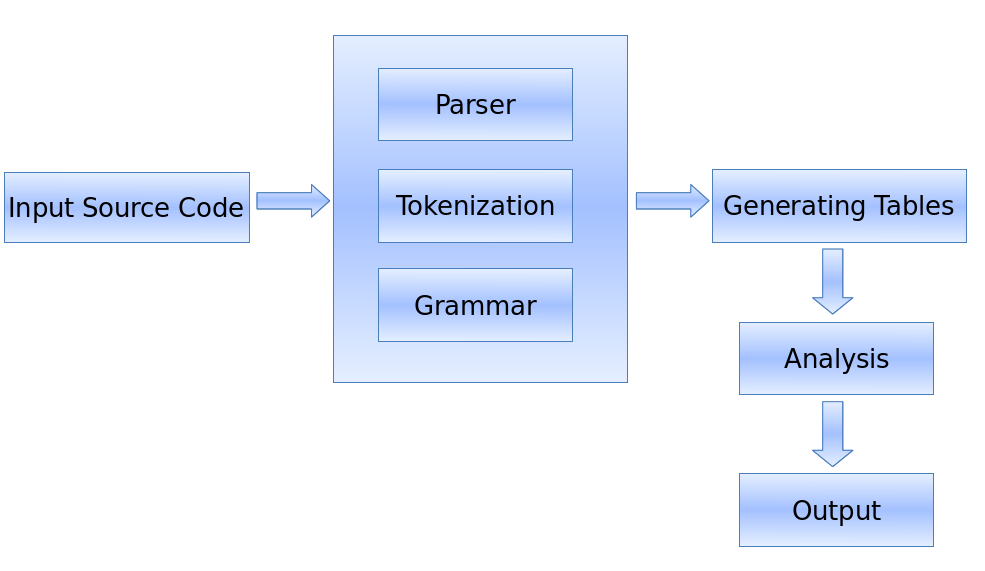
\includegraphics[scale=0.4]{architecture.png}
\caption{Architectural Diagram}
\label{<<Label>>}
\end{figure}

\section{Architecture}

\subsection{Input Source Files}
A normal multithreaded program is given as input with critical sections. This file is first compiled to check for errors and only when it is compiled error free; it heads to the next stage.
\begin{figure}[H]
\centering
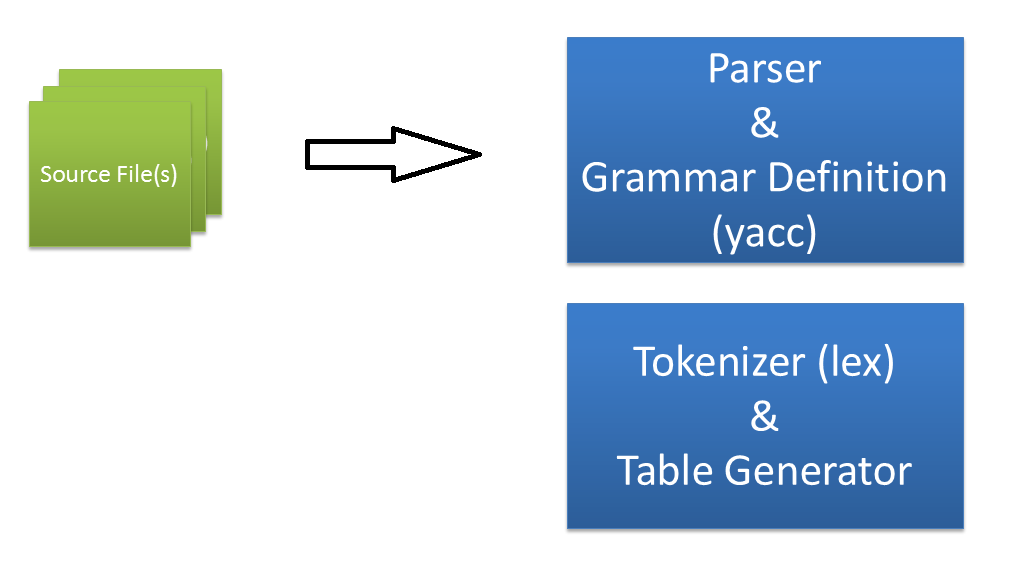
\includegraphics[scale=0.4]{input.png}
\caption{Input}
\label{<<Label>>}
\end{figure}

\subsection{Parser, Tokenizer, Grammar}
Flex (The Fast Lexical Analyser) is a tool for generating scanners. A scanner, sometimes called a tokenizer, is a program which recognizes lexical patterns in text. The flex program reads user-specified input files, or its standard input if no file names are given, for a description of a scanner to generate [4].

With it we separate all the unwanted text (ex. Comments, pre-processors) and tokenize the program to find out shared memory, functions, threads, and locks. In order to find the above from the token, it analyzes its input for occurrences of text matching the regular expressions for each rule. Whenever it finds a match, it executes the corresponding code [3].

The different in-built functions were monitoring are:\\
\begin{itemize}
\item pthread\_create
\item pthread\_join
\item pthread\_cond\_wait
\item pthread\_cond\_signal
\item sem\_wait
\item sem\_post
\end{itemize}
\begin{figure}[H]
\centering
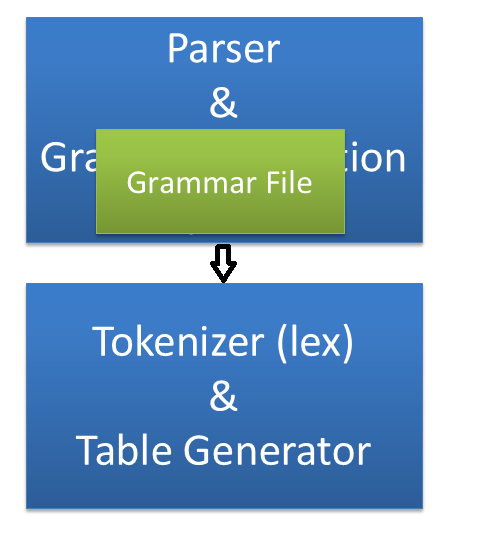
\includegraphics[scale=0.4]{grammar.png}
\caption{Parsing}
\label{<<Label>>}
\end{figure}


\subsection{Generating Tables}
Yacc (Yet Another Compiler Compiler) provides a general tool for describing the input to a computer program. We specify the structures of the input, together with code to be invoked as each such structure is recognized. Yacc turns such a specification into a subroutine that handles the input process; frequently, it is convenient and appropriate to have most of the flow of control in the user's application handled by this subroutine.

The input subroutine produced by Yacc calls a usersupplied routine to return the next basic input item. Thus, the user can specify his input in terms of individual input characters or in terms of higher level constructs such as names and numbers. The user-supplied routine may also handle idiomatic features such as comment and continuation conventions, which typically defy easy grammatical specification [5]. 

Once all the unwanted text is ignored from the code, with the help of Yacc we generate the following data structures:

\begin{itemize}
\item Global variables’ table (Id, access, variable\_name, line\_number)\\
Stores the entries of all the shared variables that exist in the program

\item User-defined Functions (Id, function\_name, return\_type, number\_of\_parameters, line\_number)\\
Stores the entries of all the functions defined by the user in the program.

\item Functions’ Local symbol table (Id, access\_type, name, data\_type, function\_id, line\_number)\\
Stores all the local variables associated with a function.

\item Semaphore table (id, name, function, location)\\
Stores all the locations of sem\_wait() and sem\_post functions used in the code

\item Thread table (Id, thread\_name, function\_name, function\_id, thread\_attribute, parameters, parent\_thread)\\
Stores all the threads associated with which functions and their attributes

\item Shared Memory Log table (Id, function\_name, shared\_object, scope, line\_number, thread-function\_id, thread\_id)\\
Stores a log of all variables which may cause data races and helps analysis the proof.

\item Critical Section table (Id, shared\_object, thread\_function\_index, first\_location, last\_location, function\_name)

\end{itemize}
\begin{figure}[H]
\centering
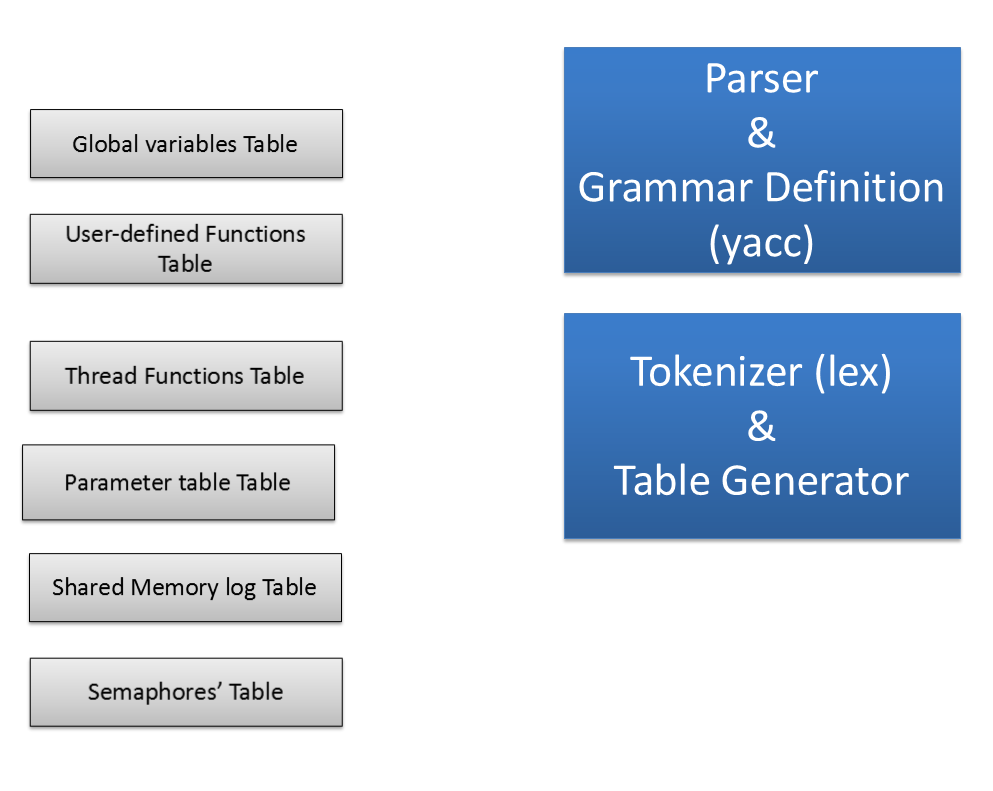
\includegraphics[scale=0.5]{tables.png}
\caption{Tables}
\label{<<Label>>}
\end{figure}

\subsection{Analysis}
Once all tables are generated we analyze them. If any shared variable exists in multiple functions and is unhandled i.e. it is not protected with the function calls sem\_wait(), sem\_post(), then we categorize that shared variable as unhandled critical section and add its entry to the critical section table.

After getting a table having all the unhandled critical sections, we analyze it for the location where we need to provides locks and unlocks. 

From the Critical Section Table, we get the line numbers of first and last occurrence of shared variables’ usage. Depending on their closeness, we decide the number of times we need to lock, and unlock.

\subsection{Output}
Once all tables are analyzed and we display all the unhandled critical sections that exist. The various attributes of the critical sections that are found are: 
\begin{itemize}

\item The shared object which is being accessed my multiple threads

\item The threads which are accessing the same shared object

\item The functions in which the critical section exist

\item The location pertaining to the line number of the critical section

\end{itemize}

\begin{figure}[H]
\centering
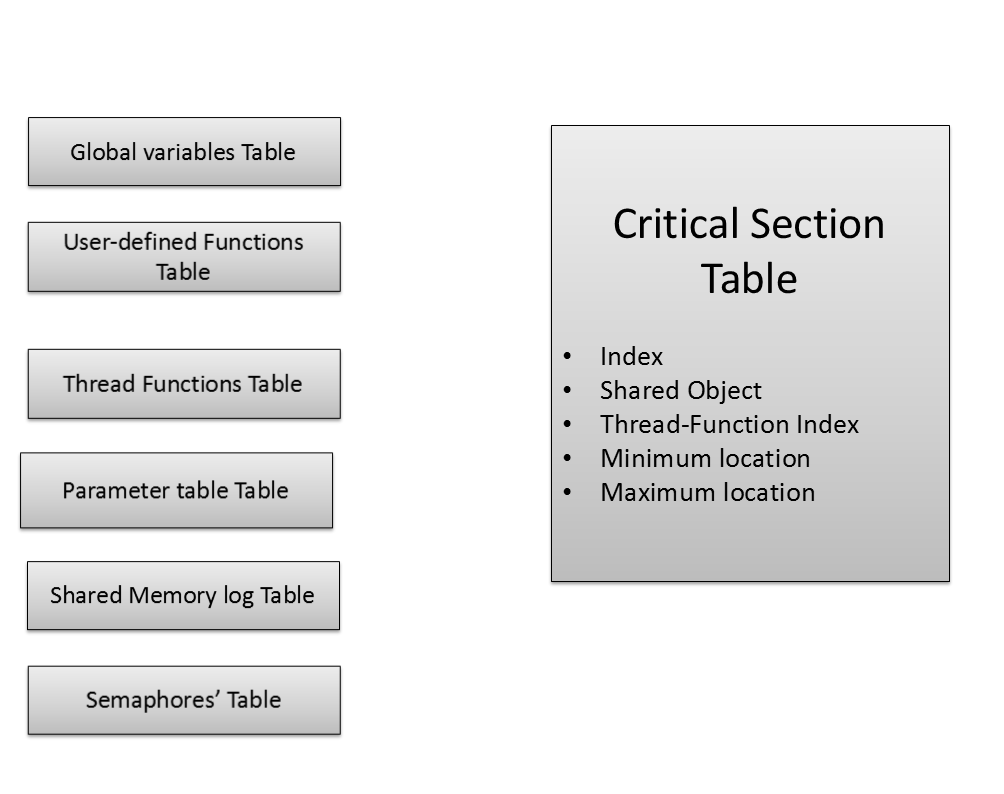
\includegraphics[scale=0.5]{cs.png}
\caption{Contents of Critical Section Table}
\label{<<Label>>}
\end{figure}

We then decide if the programmer handles the critical sections himself, or we have to handle it. Once the permissions are given, we add sem\_wait() sem\_post(), recompile the code to produce bug free programs.

\section{Placement of our tool in GCC hierarchy}
Our tool exists adjacent to the current architecture of GCC but runs once the compilation is over and no errors are generated. It keeps a copy of the original source code, works on it, and pushes its warnings along with the warnings of the compiler.
\begin{figure}[H]
\centering
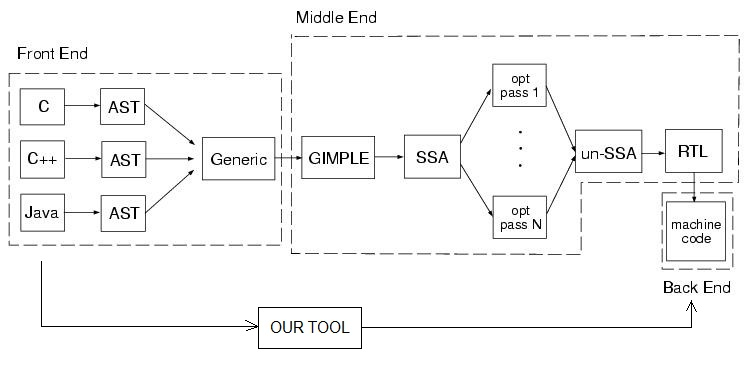
\includegraphics[scale=0.6]{gcc.jpg}
\caption{Integration of our tool in GCC}
\label{<<Label>>}
\end{figure}


 % adds the Research Methodology page
\chapter{Project Design}

\section{Software Requirement Specification}

\subsection{Hardware Requirements}
\\
\begin{itemize}
\item {2.4GHz Celeron Processor}
\item {256MB Memory}
\item {10GB Disk Space}
\end{itemize}

\subsection{Software Requirements}
\\
\begin{itemize}
\item {[Operating System]: Linux Based Operating System}
\item {[Build-essential]: Build-essential is required to build Debian packages, starting with dpkg (\textgreater= 1.14.18)}
\item {[Necessary packages for building GCC]:\\ \url{http://gcc.gnu.org/install/prerequisites.html}}
\end{itemize}

\subsection{Technologies Used}
\\
\begin{itemize}
\item C, lex, yacc.
\end{itemize}
\newpage
\section{U.M.L. Diagrams}

\subsection{Use Case}
\begin{figure}[H]
\centering
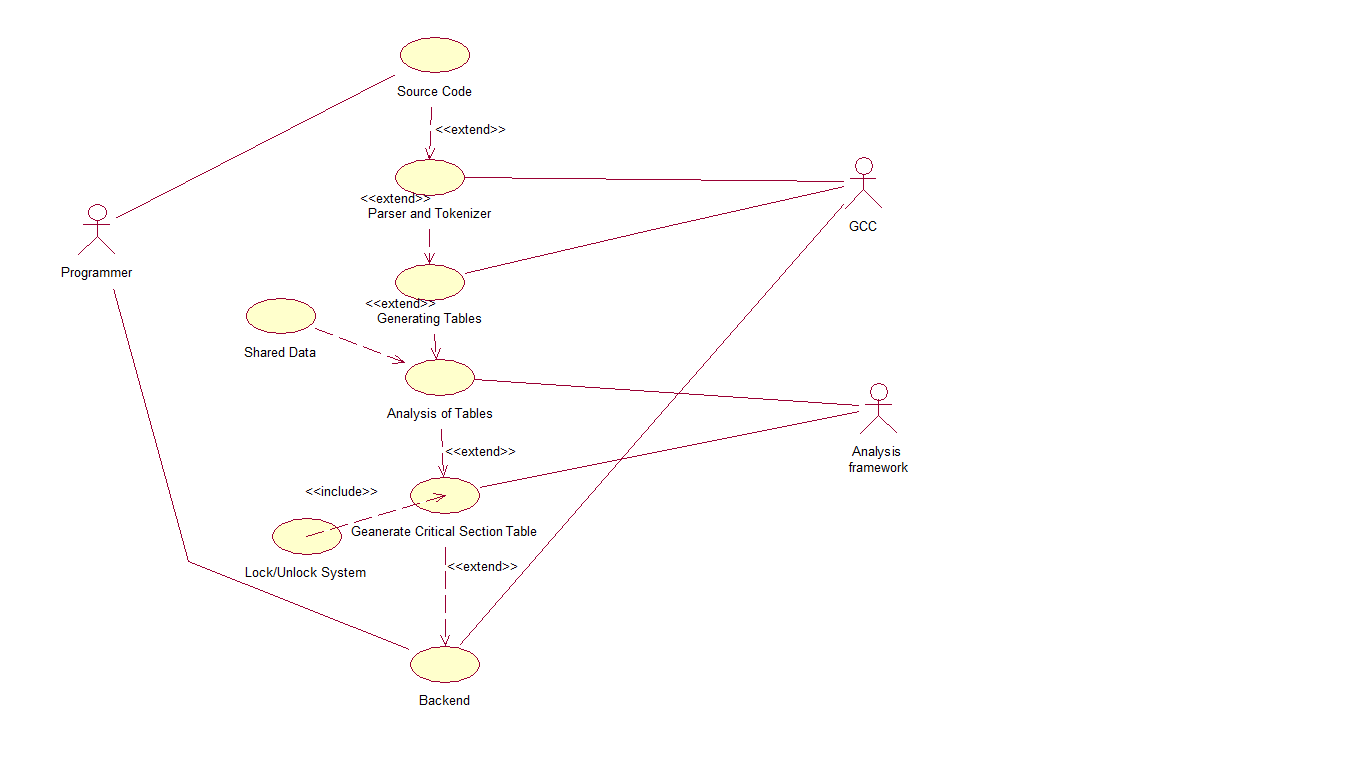
\includegraphics[scale=0.6]{usecase.png}
\caption{Use case diagram}
\label{<<Label>>}
\end{figure}
\paragraph{}
From use case point of view our system contains one actor as user or programmer, in which programmer has to specify a C source code (Source code should be error free and Multithreaded for better results).
And on the other hand GCC does the parsing and tokenization with the help of patterns and grammar that we have written, Analysis framework does the detection of critical sections in a source code provided by the Programmer as a input.


\subsection{State Chart}
\begin{figure}[H]
\centering
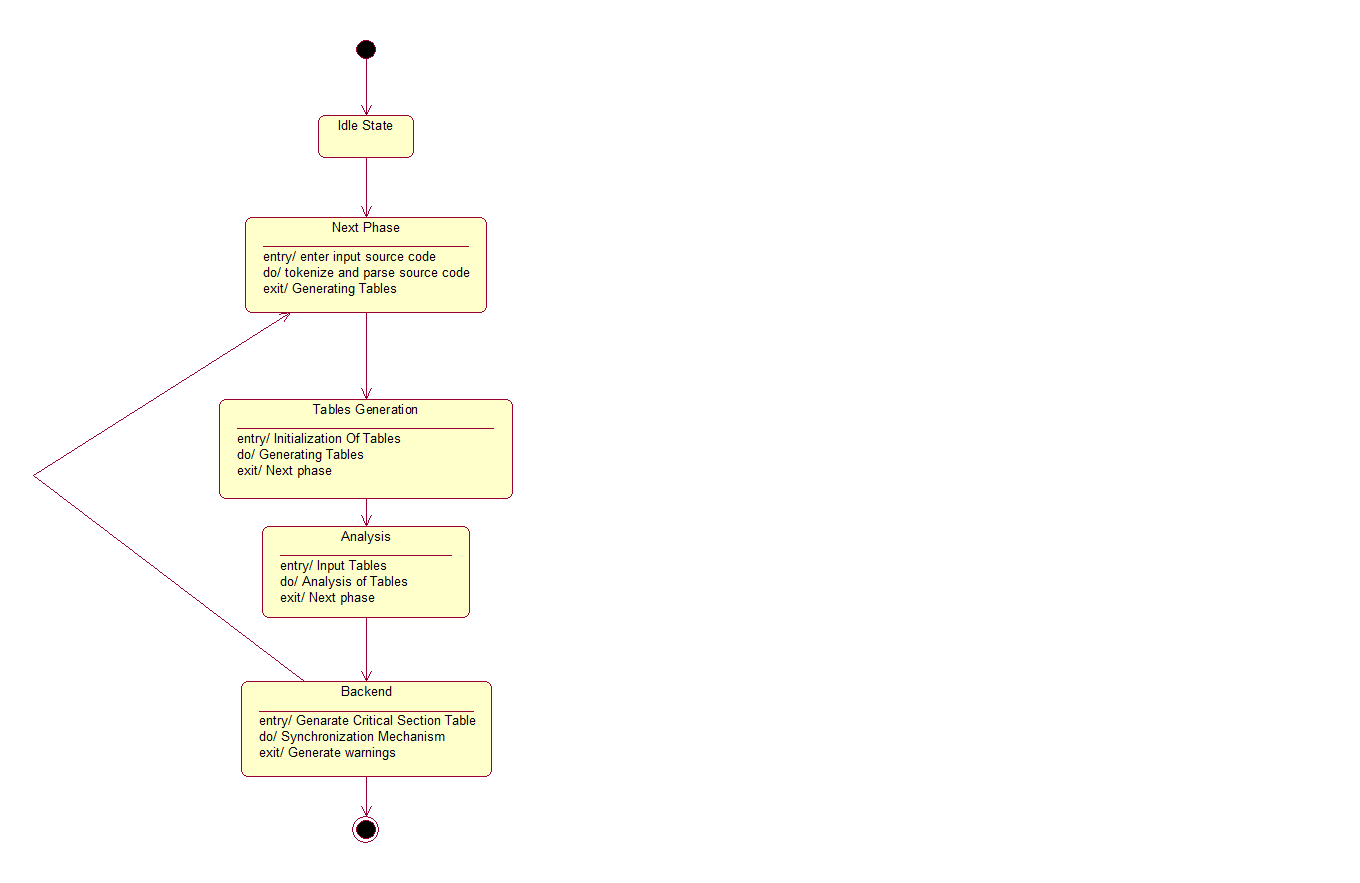
\includegraphics[scale=0.7]{statechart.png}
\caption{State chart diagram}
\label{<<Label>>}
\end{figure}
\paragraph{}
Control Flow of the Critical Section Detection System.
Above figure shows the state transisions of our system, this shows that how actually the system is going to transfer from eact step to next step after providing certain input. There are certain steps in each state. Flow of the Critical Section Detection System.

\subsection{Sequence Diagram}
\begin{figure}[H]
\centering
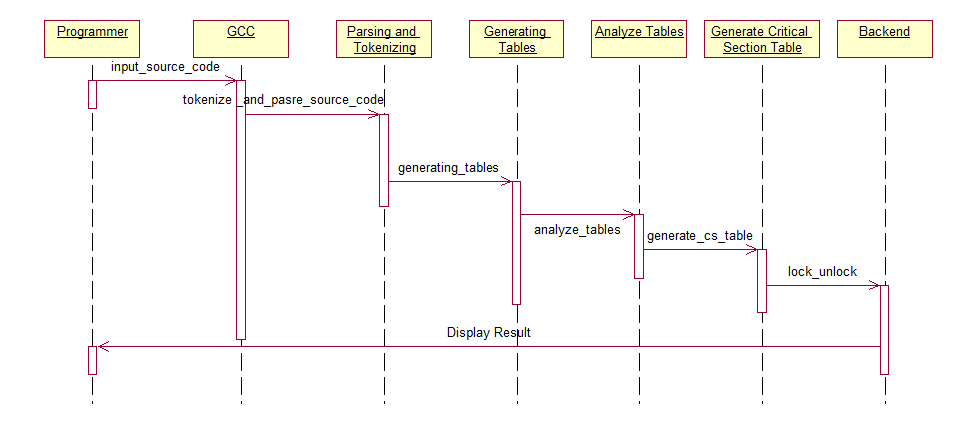
\includegraphics[scale=0.5]{sequence.png}
\caption{Sequence Diagram}
\label{<<Label>>}
\end{figure}
\paragraph{}
Shows the sequences of operations from starting to last one. A sequence diagram shows object interactions arranged in time sequence. It depicts the objects and classes involved in the scenario i.e Programmer, GCC, Analysis Framework etc. and the sequence of messages exchanged between the objects needed to carry out the functionality of the scenario. Scenario could be whole sequence of operations till the end result.  

\subsection{Collaboration Diagram}
\begin{figure}[H]
\centering
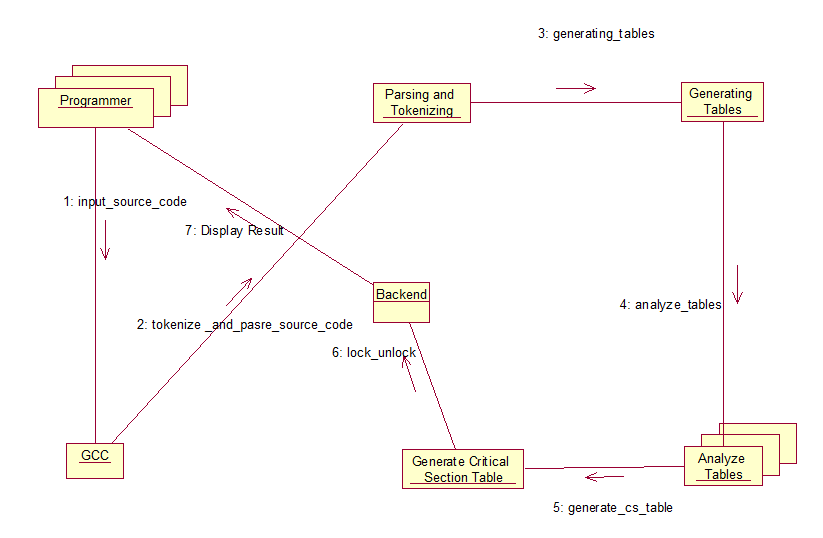
\includegraphics[scale=0.6]{collaboration.png}
\caption{Collaboration Diagram}
\label{<<Label>>}
\end{figure}
\paragraph{}
From Collaboarative perspective of our system, it covers the same scenario as shown in Sequence diagram.Indeed the collaborative view of the system is generated by using sequence diagram. 

\subsection{Activity Diagram}
\begin{figure}[H]
\centering
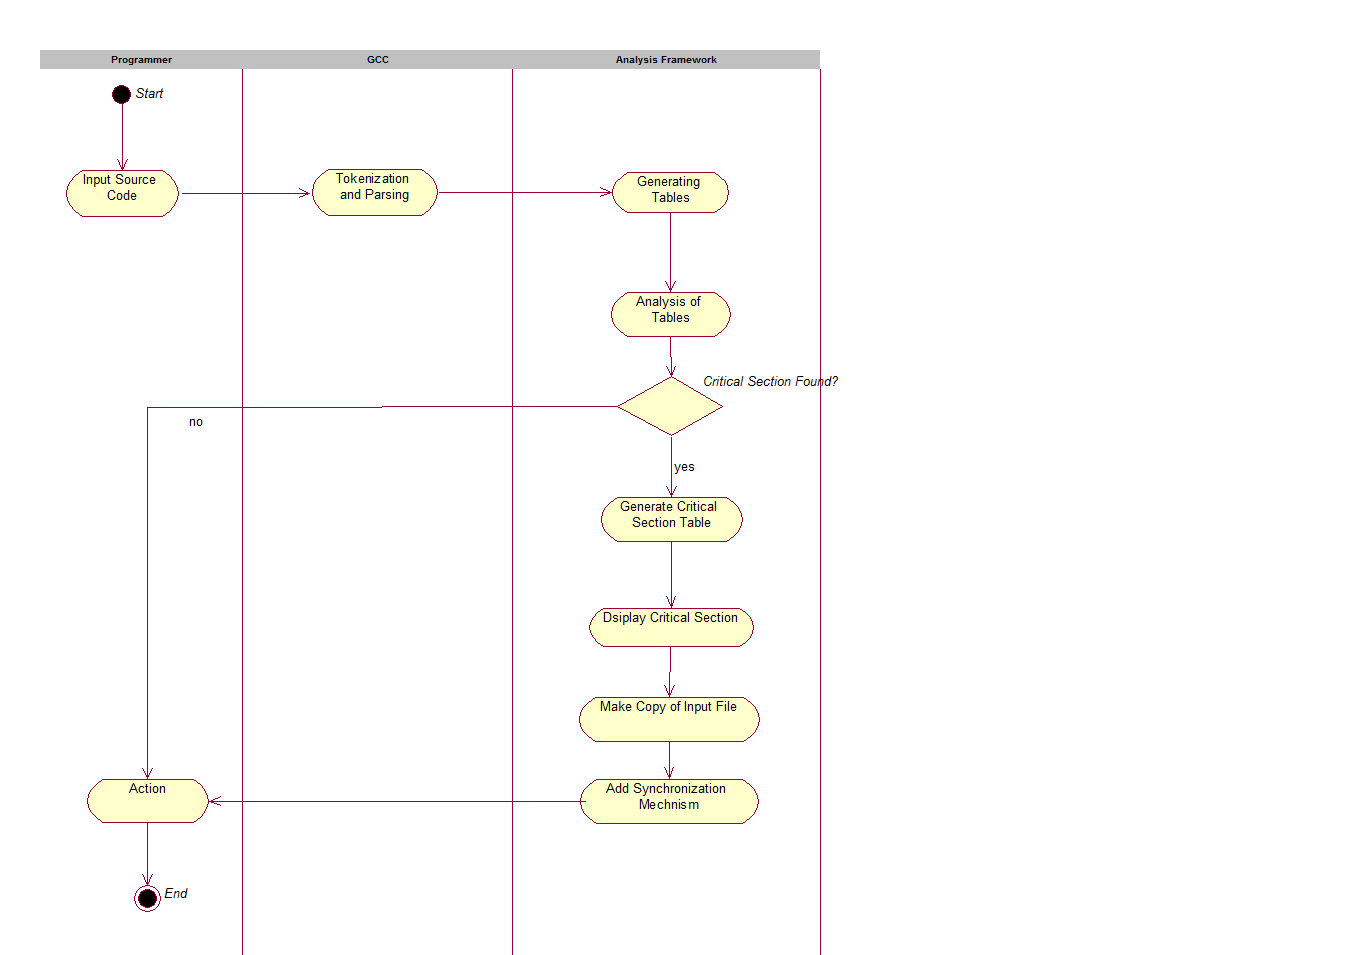
\includegraphics[scale=0.6]{activity.png}
\caption{Activity Diagram}
\label{<<Label>>}
\end{figure}
\paragraph{}
From programmers prespective activity diagram shows which are the diffrent activities performed by Programmer, GCC and the Analysis Framework.

\subsection{Component Diagram}
\begin{figure}[H]
\centering
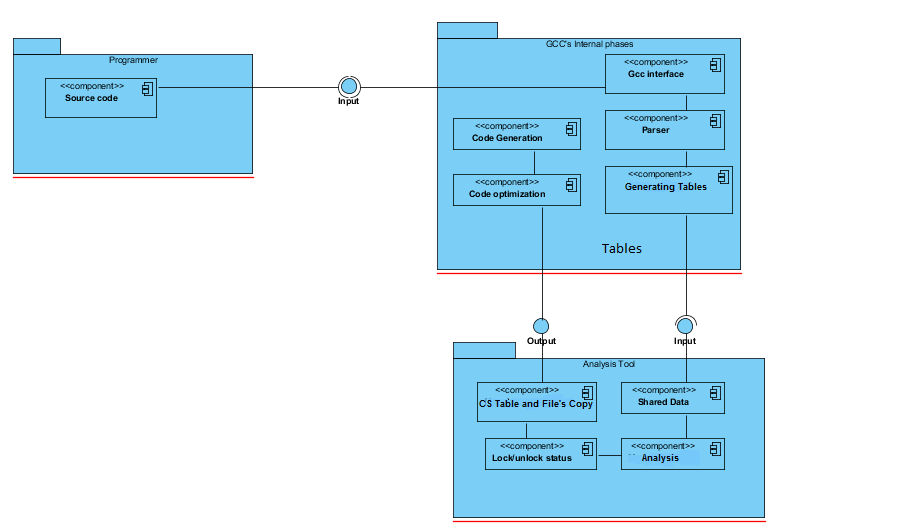
\includegraphics[scale=0.6]{component.png}
\caption{Component Diagram}
\label{<<Label>>}
\end{figure}
\paragraph{}
From Component point of view our system having different components used in system like system is Table Generator which generates the tables like Global Symbol's Table, Local Symbol's Table, Log Table, Semaphore Table, Function Table and Thread Table etc.

\subsection{Deployment Diagram}
\begin{figure}[H]
\centering
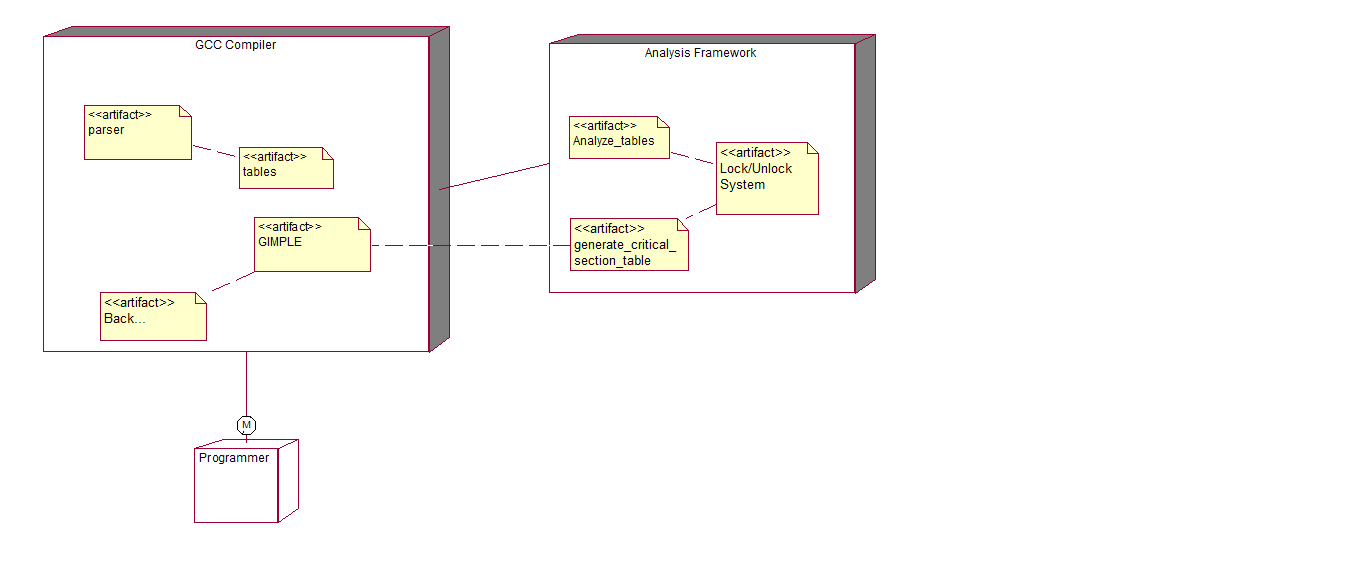
\includegraphics[scale=0.6]{deployment.png}
\caption{Deployment Diagram}
\label{<<Label>>}
\end{figure}
\paragraph{}
From deployment point of view our system contains following hardware and software component which are required for system execution are like GCC Compiler for compiling the source code, lex and yacc for Tokenization and Parsiing and the analysis frmaework for detecting the critical sections and adding synchronization mechanism.
 % adds the Project Design
\chapter{Implementation}

The important aspect of the approach is that we are analyzing the programs statically. This helps us check each and every possible case that may occur during execution of the programs. To implement the current idea of detecting critical sections, we have designed architecture as follows.


\begin{figure}[H]
\centering
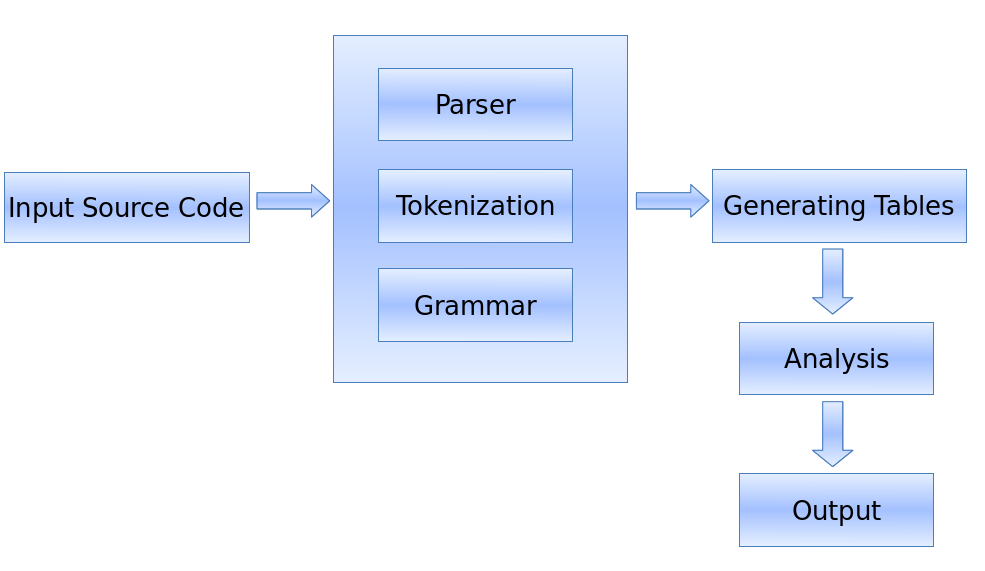
\includegraphics[scale=0.4]{architecture.png}
\caption{Architectural Diagram}
\label{<<Label>>}
\end{figure}
\newpage
\section{Architecture}

\subsection{Input Source Files}
A normal multithreaded program is given as input with critical sections. This file is first compiled to check for errors and only when it is compiled error free; it heads to the next stage.

\begin{figure}[H]
\centering
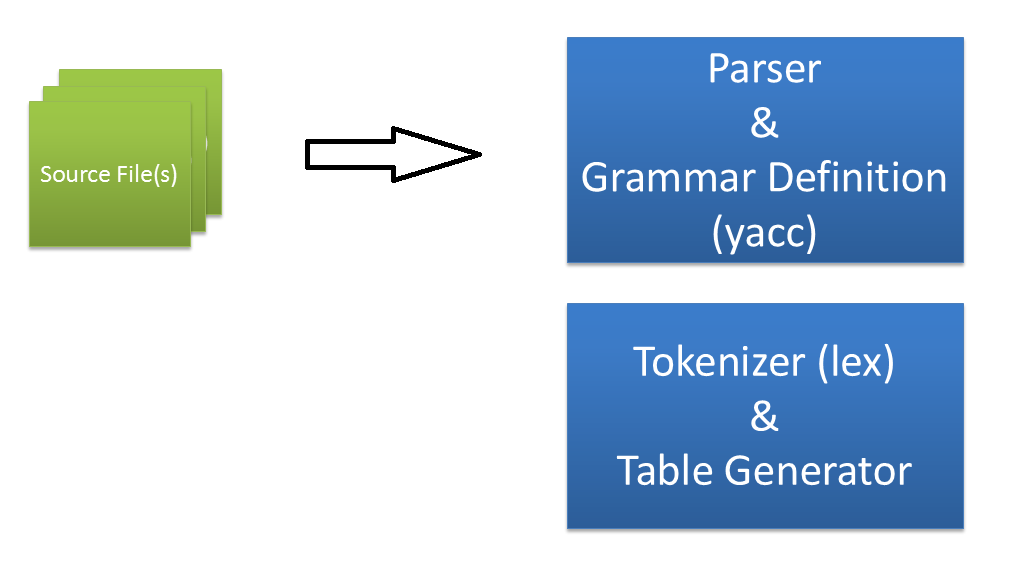
\includegraphics[scale=0.5]{input.png}
\caption{Source File(s)}
\label{<<Label>>}
\end{figure}


\subsection{Parser, Tokenizer, Grammar}
Flex (The Fast Lexical Analyser) is a tool for generating scanners. A scanner, sometimes called a tokenizer, is a program which recognizes lexical patterns in text. The flex program reads user-specified input files, or its standard input if no file names are given, for a description of a scanner to generate [4].

With it we separate all the unwanted text (ex. Comments, pre-processors) and tokenize the program to find out shared memory, functions, threads, and locks. In order to find the above from the token, it analyzes its input for occurrences of text matching the regular expressions for each rule. Whenever it finds a match, it executes the corresponding code [3].

The different in-built functions were monitoring are:\\
\begin{itemize}
\item pthread\_create\\
\item pthread\_join\\
\item pthread\_cond\_wait\\
\item pthread\_cond\_signal\\
\item sem\_wait\\
\item sem\_post\\
\end{itemize}

\begin{figure}[H]
\centering
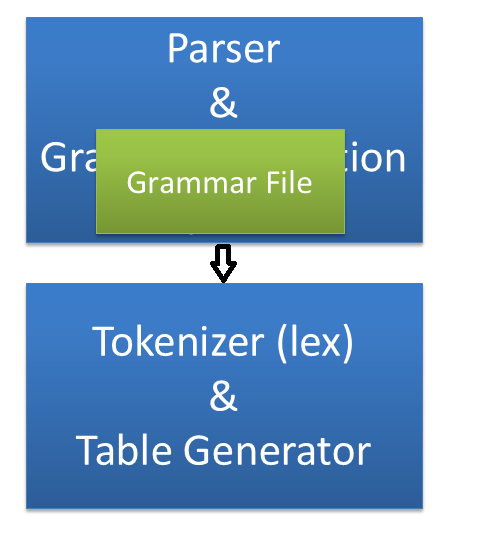
\includegraphics[scale=1]{grammar.png}
\caption{Parser, Tokenizer, Grammar}
\label{<<Label>>}
\end{figure}
\newpage
\subsection{Generating Tables}
Yacc (Yet Another Compiler Compiler) provides a general tool for describing the input to a computer program. We specify the structures of the input, together with code to be invoked as each such structure is recognized. Yacc turns such a specification into a subroutine that handles the input process; frequently, it is convenient and appropriate to have most of the flow of control in the user's application handled by this subroutine.

The input subroutine produced by Yacc calls a usersupplied routine to return the next basic input item. Thus, the user can specify his input in terms of individual input characters or in terms of higher level constructs such as names and numbers. The user-supplied routine may also handle idiomatic features such as comment and continuation conventions, which typically defy easy grammatical specification [5]. 

Once all the unwanted text is ignored from the code, with the help of Yacc we generate the following data structures:

\begin{itemize}
\item Global variables’ table (Id, access, variable\_name, line\_number)\\
Stores the entries of all the shared variables that exist in the program

\item User-defined Functions (Id, function\_name, return\_type, number\_of\_parameters, line\_number)\\
Stores the entries of all the functions defined by the user in the program.

\item Functions’ Local symbol table (Id, access\_type, name, data\_type, function\_id, line\_number)\\
Stores all the local variables associated with a function.

\item Semaphore table (id, name, function, location)\\
Stores all the locations of sem\_wait() and sem\_post functions used in the code

\item Thread table (Id, thread\_name, function\_name, function\_id, thread\_attribute, parameters, parent\_thread)\\
Stores all the threads associated with which functions and their attributes

\item Shared Memory Log table (Id, function\_name, shared\_object, scope, line\_number, thread-function\_id, thread\_id)\\
Stores a log of all variables which may cause data races and helps analysis the proof.

\item Critical Section table (Id, shared\_object, thread\_function\_index, first\_location, last\_location, function\_name)

\end{itemize}

\begin{figure}[h]
\centering
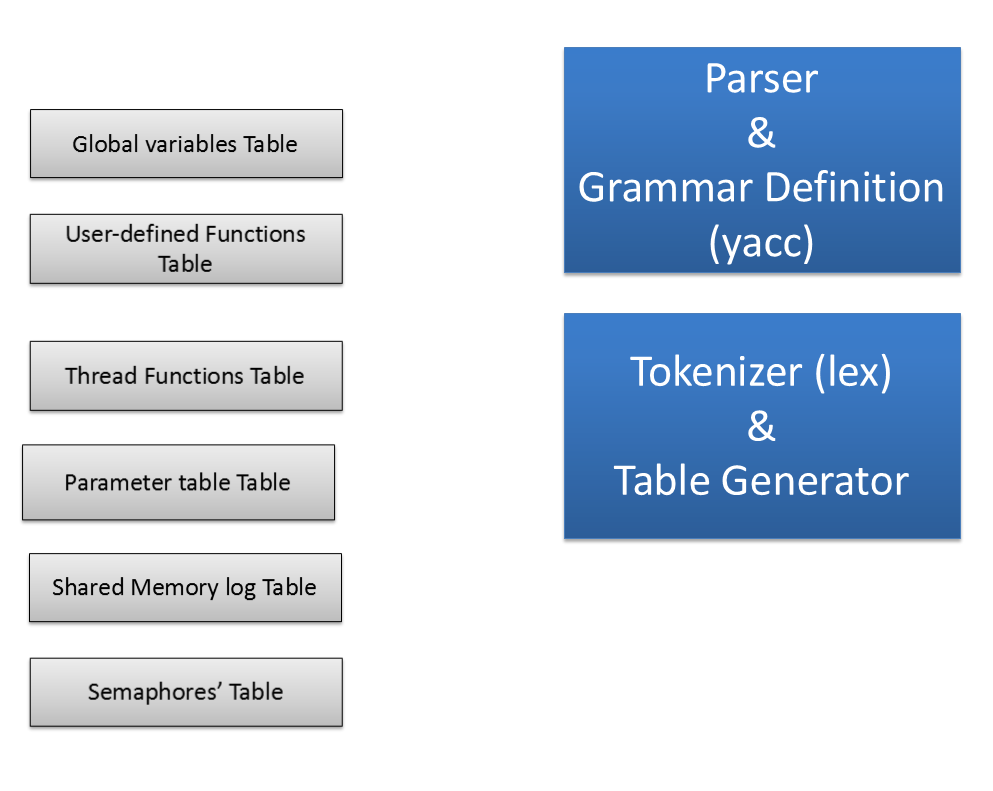
\includegraphics[scale=0.6]{tables.png}
\caption{Generated tables}
\label{<<label>>}
\end{figure}

\newpage
\subsection{Analysis}
Once all tables are generated we analyze them. If any shared variable exists in multiple functions and is unhandled i.e. it is not protected with the function calls sem\_wait(), sem\_post(), then we categorize that shared variable as unhandled critical section and add its entry to the critical section table.

After getting a table having all the unhandled critical sections, we analyze it for the location where we need to provides locks and unlocks. 

From the Critical Section Table, we get the line numbers of first and last occurrence of shared variables’ usage. Depending on their closeness, we decide the number of times we need to lock, and unlock.
\begin{figure}[h]
\centering
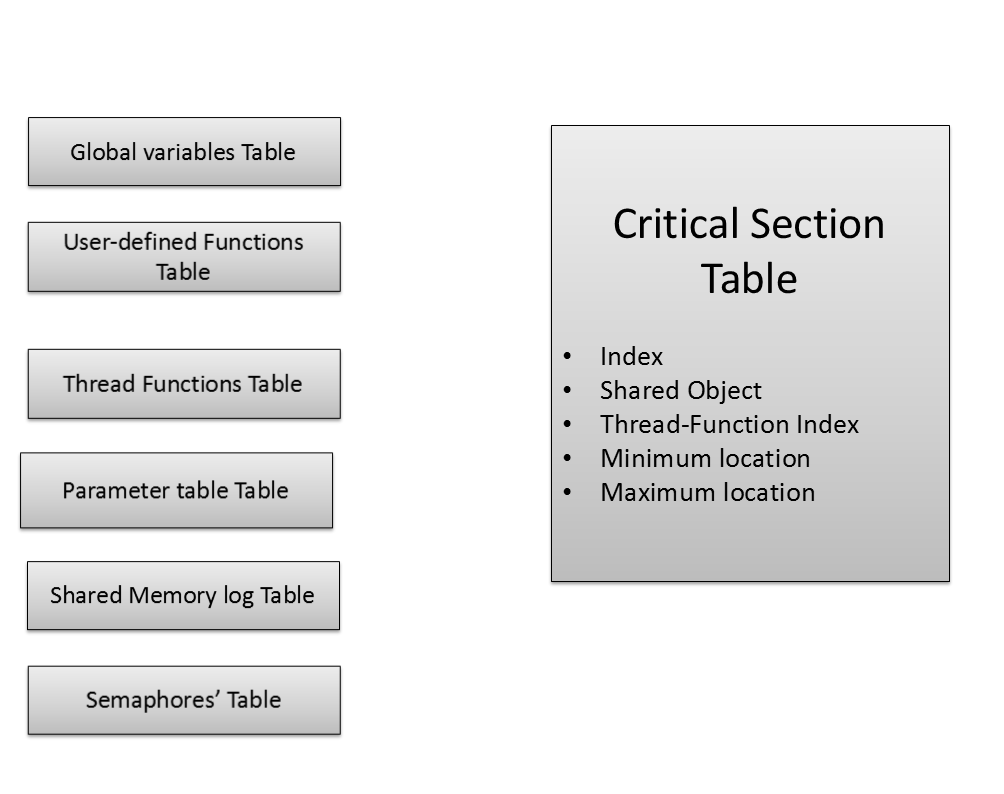
\includegraphics[scale=0.6]{cs.png}
\caption{Critical Section Table}
\label{<<label>>}
\end{figure}


\subsection{Output}
Once all tables are analyzed and we display all the unhandled critical sections that exist. The various attributes of the critical sections that are found are: 
\begin{itemize}

\item The shared object which is being accessed my multiple threads
\item The threads which are accessing the same shared object
\item The functions in which the critical section exist
\item The location pertaining to the line number of the critical section

\end{itemize}

We then decide if the programmer handles the critical sections himself, or we have to handle it. Once the permissions are given, we add sem\_wait() sem\_post(), recompile the code to produce bug free programs.

As par the implementation part is concern we required certain modules to be integrate to form the whole system or tool. Form the implementation point of view this tool is divided into following modules .
\begin{itemize}
\item Input Source File
\item Tokenization and Parsing
\item Generating Tables
\item Analysis
\item Output
\end{itemize}

%Add Description here.. 
Module of the Tokenization and Parsing

\begin{figure}[H]
\centering
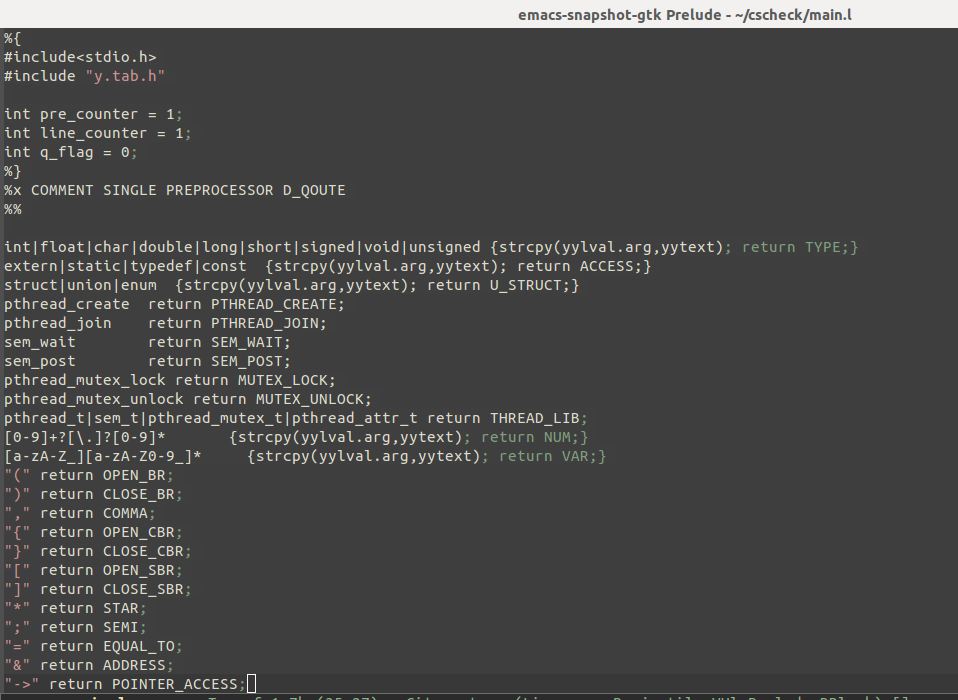
\includegraphics[scale=0.4]{Snaps/main_l_1.png}
\caption{Tokens}
\label{<<Label>>}
\end{figure}

\begin{figure}[H]
\centering
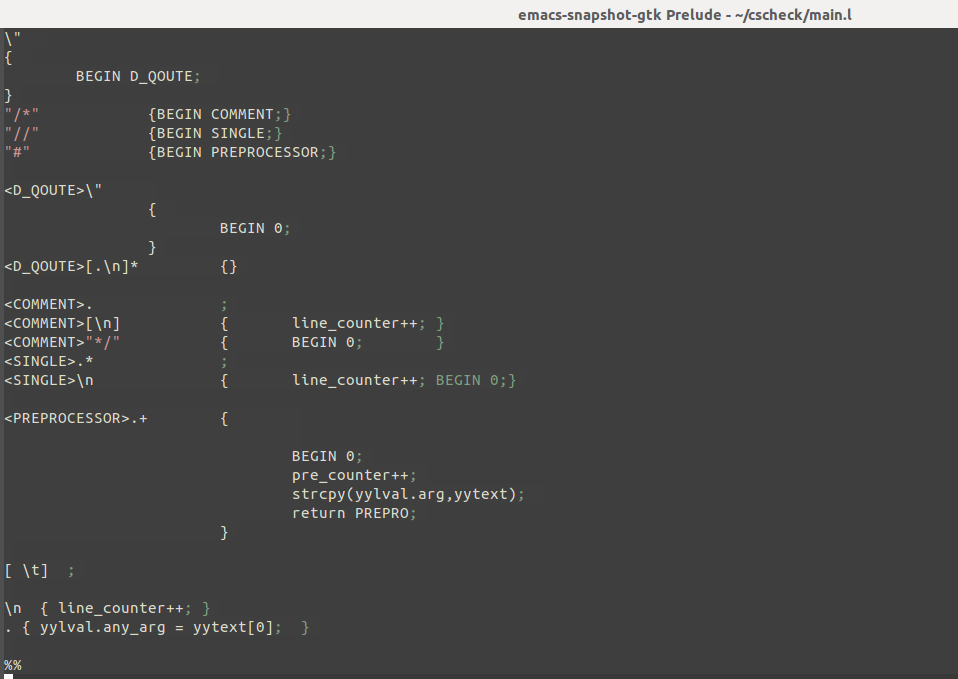
\includegraphics[scale=0.4]{Snaps/main_l_2.png}
\caption{Tokens}
\label{<<Label>>}
\end{figure}


\section{Generating Tables}
%Add Description here..
\begin{figure}[H]
\centering
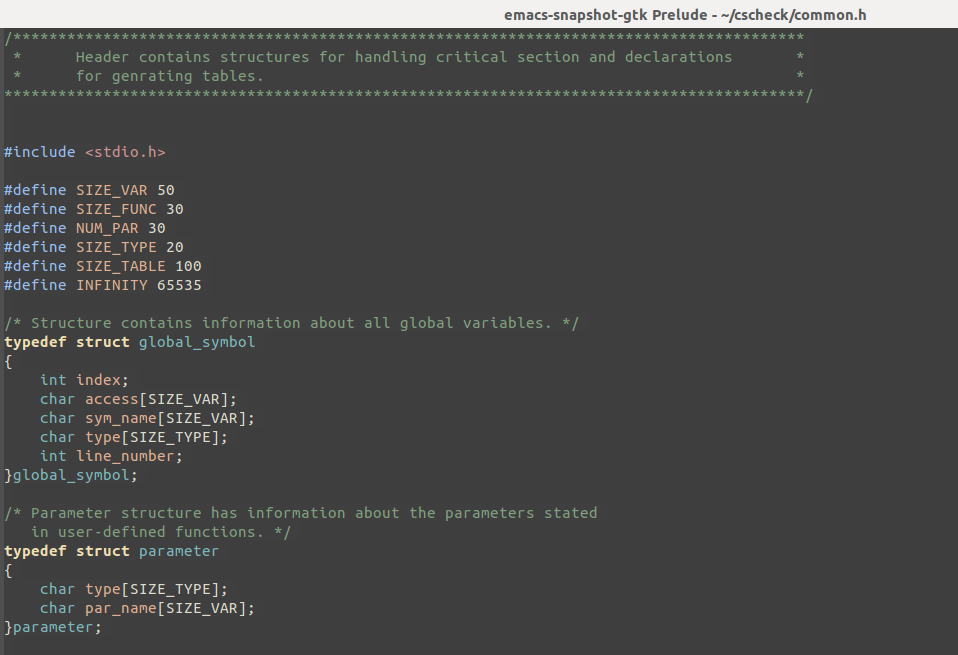
\includegraphics[scale=0.4]{Snaps/common_1.png}
\caption{Table's structure}
\label{<<Label>>}
\end{figure}
\begin{figure}[H]
\centering
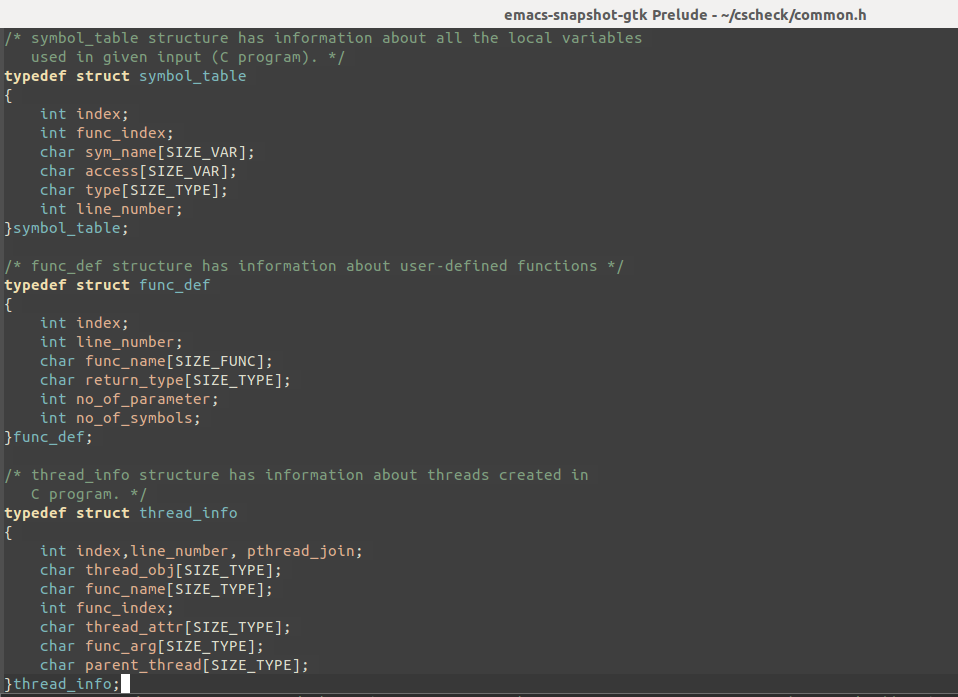
\includegraphics[scale=0.4]{Snaps/common_2.png}
\caption{Table's structure}
\label{<<Label>>}
\end{figure}

\section{Output}
%Add Description here..\begin{itemize}

If the input program is one of the following kind, then it can be said to be a correct program:
\item The shared object which is being accessed my multiple threads

\item The threads which are accessing the same shared object

\item The functions in which the critical section exist

\item The location pertaining to the line number of the critical section
\end{itemize}

\begin{figure}[H]
\centering
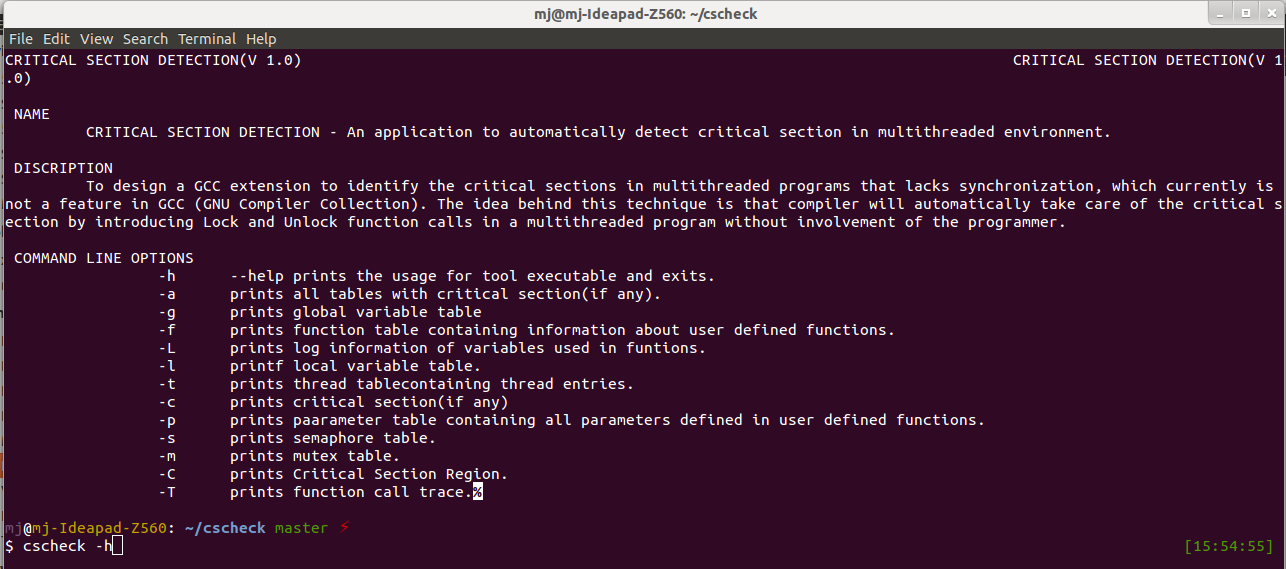
\includegraphics[scale=0.3]{Snaps/help.png}
\caption{All functionality available by different command line flags}
\label{<<Label>>}
\end{figure}


\begin{figure}[H]
\centering
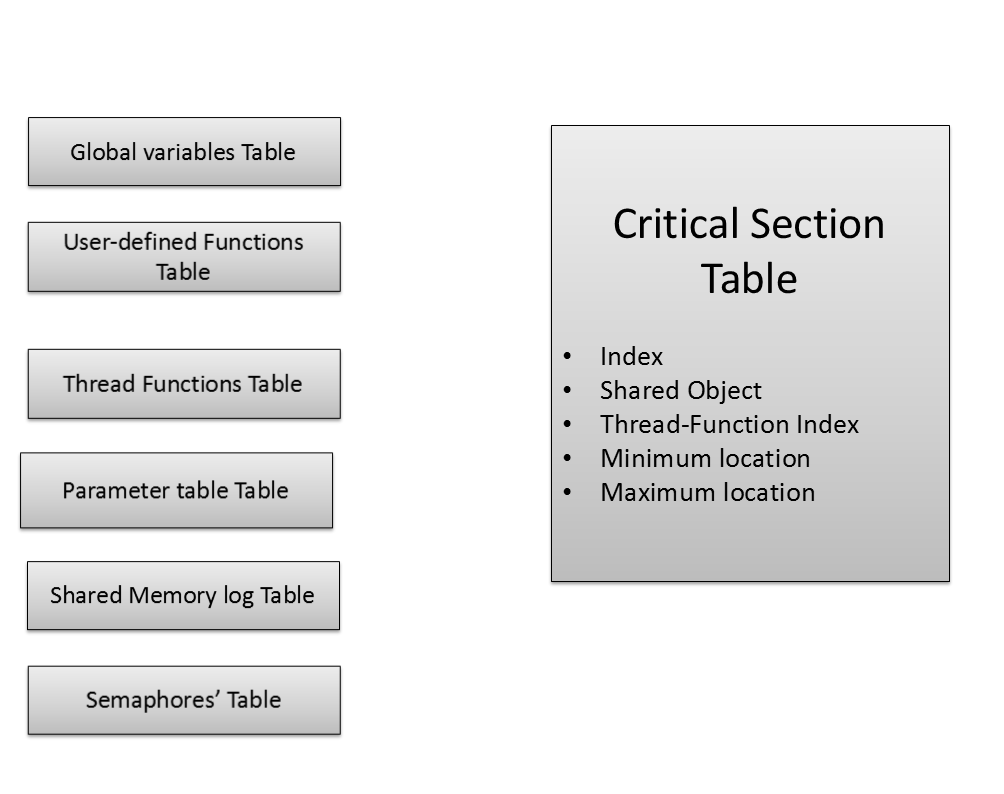
\includegraphics[scale=0.5]{cs.png}
\caption{Contents of Critical Section Table}
\label{<<Label>>}
\end{figure}

\begin{figure}[H]
\centering
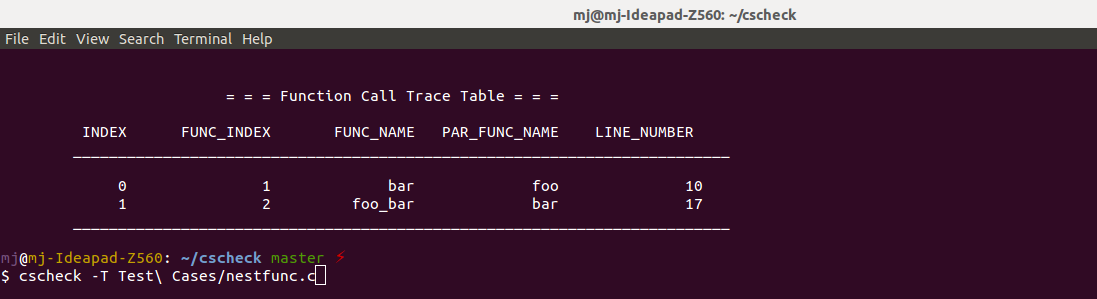
\includegraphics[scale=0.4]{Snaps/out1.png}
\caption{Call trace for a thread function}
\label{<<Label>>}
\end{figure}
\begin{figure}[H]
\centering
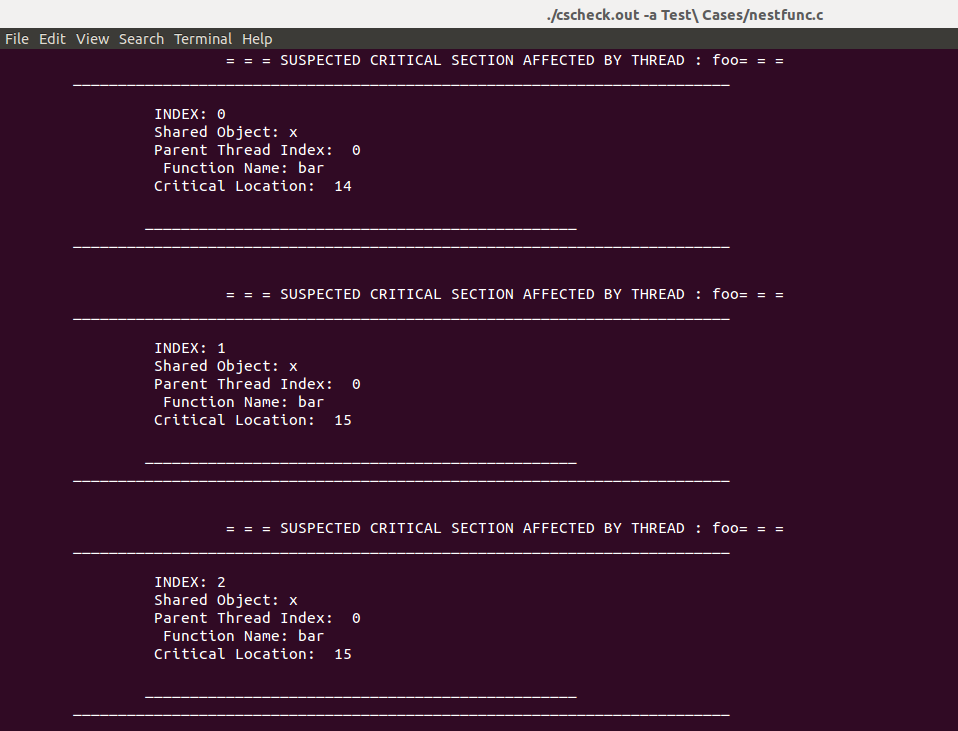
\includegraphics[scale=0.4]{Snaps/out2.png}
\caption{Detected Critical Section}
\label{<<Label>>}
\end{figure}
\begin{figure}[H]
\centering
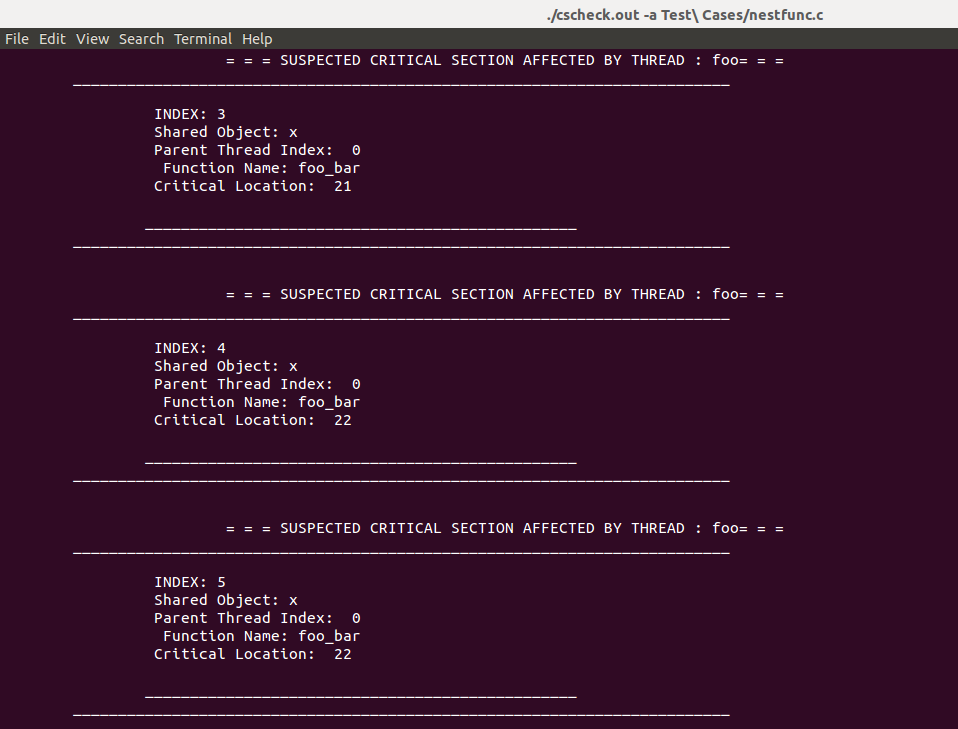
\includegraphics[scale=0.4]{Snaps/out3.png}
\caption{Suspected Critical Section}
\label{<<Label>>}
\end{figure}

\newpage
\section{Manual Testing}

% ACTUAL TABLE CODE
\setlength{\tabcolsep}{10pt}
\renewcommand{\arraystretch}{1.6}
\begin{longtable}{| p{1.9cm} | p{2.0cm} | >{\centering\arraybackslash}m{0.7cm} | p{2.1cm} | p{2.1cm} | p{1.5cm} | p{0.8cm} | }

\caption{Manual Testing}
\label{<<Label>>}
\hline
TestCase ID&Objective&Case&Procedure&Expected Results&Actual Results&Pass /Fail\\
\hline
\endfirsthead
\multicolumn{7}{c}%
{\tablename\ \thetable\ -- \textit{Continued from previous page}} \\
\hline
TestCase ID&Objective&Case&Procedure&Expected Results&Actual Results&Pass /Fail\\
\hline
\endhead
\hline \multicolumn{7}{r}{\textit{Continued on next page}} \\
\endfoot
\hline
\endlastfoot
Check Tools		& To check requirements of different tools. & 1. & a) Open Terminal and enter gcc. & GCC should be available.  & Same as Expected  & Pass \\
		&		&   & b) Open terminal and enter lex  & lex should be available   & Same as Expected   &  Pass  \\ 
		&		&   & c) Open terminal and enter yacc & yacc should be available   & Same as Expected   &  Pass  \\ \hline
  
Program Structure & To check nature of program. & 1. & a) Program should be errorless. & Compilation of program should be successful  & Same as Expected  & Pass \\
		&		&   & b) Program should contains POSIX threads. & Program should create new threads using POSIX API.   & Same as Expected   &  Pass  \\ \hline 

Tokenization & To create different tokens as per constraints. & 1. & a) Datatypes & Different tokens should be generated according to datatypes.  & Same as Expected  & Pass \\  
	     & & 2. & a) Function signature should be tokenized. & Fuction name,number of argument and return type should be tokenized  & Same as Expected  & Pass \\
	     & & 3. & b) POSIX thread's signature should be tokenized. & Thread object,Function name which is executed by thread,number of argument and return type should be tokenized  & Same as Expected  & Pass \\	
	     & & 4. & c) Semaphore signature should be tokenized. & Semaphore name,different semaphore signals should be tokenized  & Same as Expected  & Pass \\
     	     & & 5. & d) mutex signature should be tokenized. & Mutex name,different mutex signals should be tokenized  & Same as Expected  & Pass \\ \hline
	
Parsing & Generate different grammer as per tokens. & 1. & a) Grammer for variable datatypes. & Valid grammer should be generated for datatype.  & Same as Expected  & Pass \\  
	     & & 2. & b) Grammer for function signature. & Valid grammer should be generated for functions. & Same as Expected  & Pass \\
	     & & 3. & c) Grammer for POSIX thread's signature. & Valid grammer should be generated for threads. & Same as Expected  & Pass \\	
	     & & 4. & d) Grammer for API of Semaphore. & Valid grammer should be generated for semaphores & Same as Expected  & Pass \\
     	     & & 5. & e) Grammer for Mutex. & Valid grammer should be generated for mutex & Same as Expected  & Pass \\ \hline

Table Generation.& Different table are genereted according grammers. & 1. & a) Table for variable including global and local. & Valid tables should be generated for datatype including local and global.  & Same as Expected  & Pass \\  
	     & & 2. & b) Table for function signature. & Valid table should be generated for functions. & Same as Expected  & Pass \\
	     & & 3. & c) Table for POSIX thread's signature. & Valid table should be generated for threads. & Same as Expected  & Pass \\	
	     & & 4. & d) Table for API of Semaphore. & Valid table should be generated for semaphores & Same as Expected  & Pass \\
     	     & & 5. & e) Table for shared memory (Log Table ) & Valid table should be generated for shared memory & Same as Expected & Pass \\
             & & 6. & f) Table for Mutex. & Valid table should be generated for mutex & Same as Expected  & Pass \\ \hline 

Analysis of critical section.& Critical sections blocks are detected  & 1.& a) Locking and unlocking mechanism. & Check wheter locking and unlocking mechanism is exist for Critical Section.  & Same as Expected  & Pass \\  
	     & & 2. & b) Critical Section detection.& If critical section isn't synchronized then add it. & Same as Expected  & Pass \\ \hline

		
		 

\end{longtable}
% ACTUAL TABLE CODE END

 % adds the Project Design
\chapter{Testing}

% ACTUAL TABLE CODE
\setlength{\tabcolsep}{10pt}
\renewcommand{\arraystretch}{1.6}
\begin{longtable}{| p{1.9cm} | p{2.0cm} | >{\centering\arraybackslash}m{0.7cm} | p{2.1cm} | p{2.1cm} | p{1.5cm} | p{0.8cm} | }
\label{<<Label>>}
\caption{Test Cases}
\label{<<Label>>}
\hline
TestCase ID&Objective&Case&Procedure&Expected Results&Actual Results&Pass /Fail\\
\hline
\endfirsthead
\multicolumn{7}{c}%
{\tablename\ \thetable\ -- \textit{Continued from previous page}} \\
\hline
TestCase ID&Objective&Case&Procedure&Expected Results&Actual Results&Pass /Fail\\
\hline
\endhead
\hline \multicolumn{7}{r}{\textit{Continued on next page}} \\
\endfoot
\hline
\endlastfoot
Check Tools		& To check requirements of different tools. & 1. & a) Open Terminal and enter gcc. & GCC should be available.  & Same as Expected  & Pass \\
		&		&   & b) Open terminal and enter lex  & lex should be available   & Same as Expected   &  Pass  \\ 
		&		&   & c) Open terminal and enter yacc & yacc should be available   & Same as Expected   &  Pass  \\ \hline
  
Program Structure & To check nature of program. & 1. & a) Program should be errorless. & Compilation of program should be successful  & Same as Expected  & Pass \\
		&		&   & b) Program should contains POSIX threads. & Program should create new threads using POSIX API.   & Same as Expected   &  Pass  \\ \hline 

Tokenization & To create different tokens as per constraints. & 1. & a) Datatypes & Different tokens should be generated according to datatypes.  & Same as Expected  & Pass \\  
	     & & 2. & a) Function signature should be tokenized. & Fuction name,number of argument and return type should be tokenized  & Same as Expected  & Pass \\
	     & & 3. & b) POSIX thread's signature should be tokenized. & Thread object,Function name which is executed by thread,number of argument and return type should be tokenized  & Same as Expected  & Pass \\	
	     & & 4. & c) Semaphore signature should be tokenized. & Semaphore name,different semaphore signals should be tokenized  & Same as Expected  & Pass \\
     	     & & 5. & d) mutex signature should be tokenized. & Mutex name,different mutex signals should be tokenized  & Same as Expected  & Pass \\ \hline
	
Parsing & Generate different grammer as per tokens. & 1. & a) Grammer for variable datatypes. & Valid grammer should be generated for datatype.  & Same as Expected  & Pass \\  
	     & & 2. & b) Grammer for function signature. & Valid grammer should be generated for functions. & Same as Expected  & Pass \\
	     & & 3. & c) Grammer for POSIX thread's signature. & Valid grammer should be generated for threads. & Same as Expected  & Pass \\	
	     & & 4. & d) Grammer for API of Semaphore. & Valid grammer should be generated for semaphores & Same as Expected  & Pass \\
     	     & & 5. & e) Grammer for Mutex. & Valid grammer should be generated for mutex & Same as Expected  & Pass \\ \hline

Table Generation.& Different table are genereted according grammers. & 1. & a) Table for variable including global and local. & Valid tables should be generated for datatype including local and global.  & Same as Expected  & Pass \\  
	     & & 2. & b) Table for function signature. & Valid table should be generated for functions. & Same as Expected  & Pass \\
	     & & 3. & c) Table for POSIX thread's signature. & Valid table should be generated for threads. & Same as Expected  & Pass \\	
	     & & 4. & d) Table for API of Semaphore. & Valid table should be generated for semaphores & Same as Expected  & Pass \\
     	     & & 5. & e) Table for shared memory (Log Table ) & Valid table should be generated for shared memory & Same as Expected & Pass \\
             & & 6. & f) Table for Mutex. & Valid table should be generated for mutex & Same as Expected  & Pass \\ \hline 

Analysis of critical section.& Critical sections blocks are detected  & 1.& a) Locking and unlocking mechanism. & Check wheter locking and unlocking mechanism is exist for Critical Section.  & Same as Expected  & Pass \\  
	     & & 2. & b) Critical Section detection.& If critical section isn't synchronized then add it. & Same as Expected  & Pass \\ \hline

		
		 

\end{longtable}
% ACTUAL TABLE CODE END
 % adds the Project Design
\chapter{Scheduling}


\section{Proposed Modules}
\begin{itemize}
\item Parse, Tokenize
\item Tables Generation
\item Analysis
\item Testing
\end{itemize}
\section{Scheduling}
 % adds the Scheduling and Planning page
\chapter{Conclusion and Future Scope}

\section{Conclusion}
The overall approach helps solve many practical problems. \\
Bugs that are notoriously difficult to find in concurrent programming are handled by the compiler itself. In large code bases data races possibilities be will perfectly identified and this framework will help automatically detect critical section and provide Lock/Unlock system without involvement of the programmer.

\section{Future Scope}
Although this concept if pretty much full proof, the capabilities can extended further.\\
As of now, we are only supporting POSIX thread library and semaphore locking mechanism, this project can be extended for other thread libraries and locking mechanism.
\begin{itemize}
\item OpenThreads
\item Boost C++ libraries http://www.boost.org/
\item OpenMP http://openmp.org/wp/
\item Intel Cilk Plus http://software.intel.com/en-us/intel-cilk-plus
\item ZThreads http://zthread.sourceforge.net/
\end{itemize}

Since this approach is generic, we can port the same for compilers of other languages. Since critical sections are one of the most important factors of concurrent programming, this port would help programmers of other domain incorporate it with their development and benefit from it.

For now we have only concentrated on shared memory in User space. A possible future enhancement could be that we can tackle shared memory in the kernel space, (for example: kernel level pipes) or handle files as well.

A very difficult (but a possible) concept of adding synchronization mechanisms automatically could be done. However, many complications are associated with it as locking mechanism depends on the application logic, which is practically impossible to identify programmatically.


 % adds the Scheduling and Planning page
\begin{thebibliography}{99}
\addcontentsline{toc}{chapter}{\bibname}
\lhead{}\markboth{\bibname}{}

% \bibitem{TEXT} is how you refer to your reference in your report. keep that very short
% \emph{Paper Name} is just to highligh the paper name by making it italic, not required but looks nice

%Example
%\bibitem{short_paper_name}\emph{Paper Name}; Author Name, Conference Name, year etc


%And how you would refer to the paper in the text - example
%Your text in other tex files \cite{short_paper_name} contd explaining

%If you have to display links, do it via adding \\ (newline) otherwise it goes off the margins. Don't know how to fix this yet
%\bibitem{short_link_name}Link Name \\ \url{http://url link here}
%\url{The-human-element-the-weakest}



\end{thebibliography}
 % adds the References page

\end{document}
